% !TeX encoding = UTF-8
% !TeX program = pdflatex
% !TeX spellcheck = en_US
\documentclass[binding=0.6cm]{sapthesis}
\usepackage{microtype}
\usepackage[english]{babel}
\usepackage[utf8]{inputenc}
\usepackage{csquotes}
\usepackage{dirtytalk}
\usepackage{amssymb,amsmath}
\usepackage{bbold}

\usepackage{setspace}
%\singlespacing
\onehalfspacing

\usepackage[backend=biber,style=apa]{biblatex}
\bibliography{bibliography}

%%%% ZAVVE: to add parenthesis to \cite{} command
\newcommand{\mycite}[1]{(\cite{#1})}

\usepackage{hyperref}
\hypersetup{
    %hyperfootnotes=true,			
    %bookmarks=true,			
    %colorlinks=true,
    %linkcolor=red,
    %linktoc=page,
    %anchorcolor=black,
    %citecolor=red,
    %urlcolor=blue,
    pdftitle={Parametrized CF Explanations in Graph Neural Networks},
    pdfauthor={Giammarco D'Alessandro},
    pdfkeywords={thesis, sapienza, roma, university}
}
\usepackage{cleveref}


\title{Parametrized Counterfactual Explanations for Node Classification in Graph Neural Networks}
\author{Giammarco D'Alessandro}
\IDnumber{1753102}
\course{Corso di laurea magistrale in Engineering in Computer Science - Ingegneria Informatica}
\courseorganizer{Facoltà di Ingengneria dell'Informazione, Informatica e Statistica}
\AcademicYear{2022/2023}
\advisor{Prof. Fabrizio Silvestri}
\coadvisor{Prof. Simone Scardapane}
\examdate{31 October 2023}
\examiner{Prof. Aristidis Anagnostopoulos,\\Prof. Antonio Cianfrani,\\Prof. Fabrizio D’Amore,\\Prof. Luca Iocchi,\\Prof. Massimo Panella,\\Prof. Gabriele Proietti Mattia,\\Prof. Leonardo Querzoni,\\Prof. Simone Scardapane,\\Prof. Fabrizio Silvestri,\\Prof. Angelo Spognardi,\\Prof. Andrea Vitaletti,\\Prof. Massimo Mecella}
\authoremail{dalessandro.1753102@studenti.uniroma1.it}
\copyyear{2023}
%\thesistype{Master thesis}

\begin{document}

\frontmatter
\maketitle
\dedication{Dedicato a\\Fulmine di Pegasus}

%%%% ZAVVE: to increase page headline space
%\setlength{\headheight}{25pt}.
%\setlength{\headsep}{12pt}.

\begin{abstract}
Given the increasing popularity of Graph Neural Networks (GNNs) in real-world applications such as computational biology, natural language processing (NLP), and computer security, etc...; and the \textit{black-box} nature of such models, several methods have been developed for explaining their predictions. One recent approach to address this problem is counterfactual reasoning, where the goal of an explainer algorithm is to induce a change in the GNN prediction by minimal perturbation of the input structure. 

%Existing methods for interpreting predictions from GNNs have primarily focused on generating subgraphs that are especially relevant for a particular prediction. However, such methods are not counterfactual (CF) in nature: given a prediction, we want to understand how the prediction can be changed in order to achieve an alternative outcome. In this work, we propose a method for generating CF explanations for GNNs: the minimal perturbation to the input (graph) data such that the prediction changes. Using only edge deletions, we find that our method, CF-GNNExplainer, can generate CF explanations for the majority of instances across three widely used datasets for GNN explanations, while removing less than 3 edges on average, with at least 94\% accuracy. This indicates that CF-GNNExplainer primarily removes edges that are crucial for the original predictions, resulting in minimal CF explanations.

%Graph neural networks (GNNs) find applications in various domains such as computational biology, natural language processing, and computer security. Owing to their popularity, there is an increasing need to explain GNN predictions since GNNs are black-box machine learning models. One way to address this is counterfactual reasoning where the objective is to change the GNN prediction by minimal changes in the input graph. Existing methods for counterfactual explanation of GNNs are limited to instance-specific local reasoning. This approach has two major limitations of not being able to offer global recourse policies and overloading human cognitive ability with too much information. In this work, we study the global explainability of GNNs through global counterfactual reasoning. Specifically, we want to find a small set of representative counterfactual graphs that explains all input graphs. Towards this goal, we propose GCFExplainer, a novel algorithm powered by vertexreinforced random walks on an edit map of graphs with a greedy summary. Extensive experiments on real graph datasets show that the global explanation from GCFExplainer provides important high-level insights of the model behavior and achieves a 46.9% gain in recourse coverage and a 9.5% reduction in recourse cost
\end{abstract}

\tableofcontents
\mainmatter

%%%%%%%%%%%%%%%%%%%%%%%%% CHAP.1 : Introduction 
\chapter{Introduction}
\label{chap:1-intro} 
In recent years, Graph Neural Networks (GNNs) have emerged as a powerful tool for analyzing complex relational data represented in the form of graphs. Graphs are pervasive in various domains, including social networks, biological systems, transportation networks, and recommendation systems. The ability of GNNs to model and understand these graph structures has led to significant advancements in tasks such as node classification, link prediction, and community detection.

%%% black box models
%%% citare GDPR e XAI: come in CF survey

Node classification, a fundamental task in graph analysis, involves predicting labels or categories for nodes in a graph based on their structural and attribute information. Despite the remarkable success of GNNs in node classification, interpreting their decisions remains a challenge. Understanding why a GNN predicts a specific label for a node is crucial for building trust, improving model robustness, and gaining insights into the underlying data.

One promising approach to address the interpretability challenge in GNNs is the integration of counterfactual explanations in eXplainable Artificial Intelligence (XAI\footnotemark). Counterfactual explanations provide meaningful insights into model predictions by identifying what changes in the input features would lead to a different prediction. In the context of node classification, counterfactual explanations can elucidate the necessary alterations to the node's attributes or connections that would result in a different predicted label.

\footnotetext{The acronym was made popular by the USA Defense Advanced Research Projects Agency when launching to the research community the challenge of designing self-explanatory AI systems (\url{https://www.darpa.mil/program/explainable-artificial-intelligence}).}


This thesis focuses on the incorporation of counterfactual explanations to enhance interpretability in GNNs for node classification. We explore how these explanations can shed light on the decision-making process of GNNs and provide actionable insights for stakeholders. The objective is to bridge the gap between predictive accuracy and model interpretability, facilitating the deployment of GNNs in real-world applications where transparency and trustworthiness are paramount.

%%% research onjectives

In this introductory chapter, we present an overview of the research problem, define the research objectives, outline the scope and contributions of this thesis, and provide a brief outline of the subsequent chapters. Additionally, we discuss the significance of counterfactual explanations in the context of GNNs and node classification, setting the stage for the subsequent chapters that delve deeper into this research domain.

\section{Thesis outline}
The subsequent chapters of this thesis are organized as follows:
\begin{itemize}
    \item \textbf{Chapter 2: Background}, provides an in-depth review of the related literature, covering topics related to deep learning and Graph Neural Networks (GNNs), exaplainable artificial intelligence and counterfactual explanations.
    \item \textbf{Chapter 3: Parametrized Counterfactual Explanations for Node Classification in Graph Neural Networks} outlines the proposed methodologies for generating counterfactual explanations for GNNs, including algorithmic details and rationales.
    \item \textbf{Chapter 4: Experimental and evaluation} presents the experimental setup, datasets, evaluation metrics, and results obtained from assessing the effectiveness of the proposed methodologies.
    \item \textbf{Chapter 5: Conclusions and future work} summarizes the contributions of the thesis, discusses limitations, and outlines potential directions for future research in this domain.
\end{itemize}




%%%%%%%%%%%%%%%%%%%%%%%%% CHAP.2 : Introduction
\chapter{Background}
\label{chap:2-background}
Understanding the context and rationale behind the research is crucial for appreciating the significance and relevance of the work presented herein. This background chapter provides an overview of the fundamental concepts, theories, and existing research relevant to Graph Neural Networks (GNNs) and eXplainable Artificial Intelligence (XAI). It sets the stage by presenting the existing knowledge landscape, highlighting key theories, models, and advancements in the field of study.

In section \ref{sec:bg.gnn} an introduction of the background theory of GNNs is presented, starting from the basis of graph theory (\cref{sec:bg.gnn.graph-base}) and the foundation of deep learning (\cref{sec:bg.gnn.DL-history}), and proceeding with a more detailed description of GNNs, and their variations (\cref{sec:bg.gnn.gnns}). In section \ref{sec:bg.xai} instead faces the other fundamental topic of this work, XAI. First an overview of the main concept in this field, explainablity and interpretability, is introduced (\cref{sec:bg.xai.inter-vs-xai}) together with some example solutions (\cref{sec:bg.xai.shap-lime}), subsequently sections \ref{sec:bg.xai.gnn-xai} and \ref{sec:bg.xai.cf-reason} deal with explainability focused on GNNs and counterfactual reasoning, respectively.

\section{Graph Neural Networks (GNNs)}
\label{sec:bg.gnn}
Graph Neural Networks (GNNs, \cite{gnnModel2009}) represent a revolutionary paradigm in the field of machine learning, particularly suited for analyzing and extracting insights from complex structured data, such as graphs. Traditional neural networks excel at processing signals like images, speech, videos or sequences in which there is an underlying Euclidean structure, but they struggle with non-Euclidean data, like graphs. Such kinds of data implies that there are no such familiar properties as global parameterization, common system of coordinates, vector space structure, or shift-invariance. Consequently, basic operations like convolution that are taken for granted in the Euclidean case are even not well defined on non-Euclidean domains \mycite{Bronstein_2017}. 

GNNs, on the other hand, have emerged as a powerful tool for handling these intricate data structures by incorporating graph-related properties. Recent developments have increased their capabilities and expressive power. Practical applications have become popular in a really wide spectrum of different areas such as drug discovery \mycite{doi:10.1021/acs.jmedchem.9b00959}, physics simulations \mycite{sanchezgonzalez2020learning}, fake news detection \mycite{monti2019fake}, recommendation systems \mycite{eksombatchai2017pixie} and many others \mycite{hamilton2020graph}.

In essence, GNNs are a class of deep learning models designed to operate on graphs, capturing both the node-level and the edge-level information within a graph. They are engineered to learn meaningful representations of nodes and edges by leveraging the graph's topology and associated features. These representations can be exploited in performing various tasks, such as node classification, link prediction, community detection, and graph generation. More generally GNNs have shown remarkable performance in domains where relationships and interactions between entities are crucial for understanding system dynamics and making informed predictions.

This introduction will delve deeper into the foundations, architectures, and applications of Graph Neural Networks, providing a comprehensive understanding of this cutting-edge approach to processing complex relational data. First it will go through some basics of graph theory and it will analyze how these concepts can be used to model real world scenarios, and how neural networks  can exploit the information encoded in such models. Last it will added a brief presentation of different types of GNNs and their peculiarities.

\subsection{From graphs to Graph Neural Networks}
\label{sec:bg.gnn.graph-base}

\begin{figure}
    \centering
    \footnotesize a)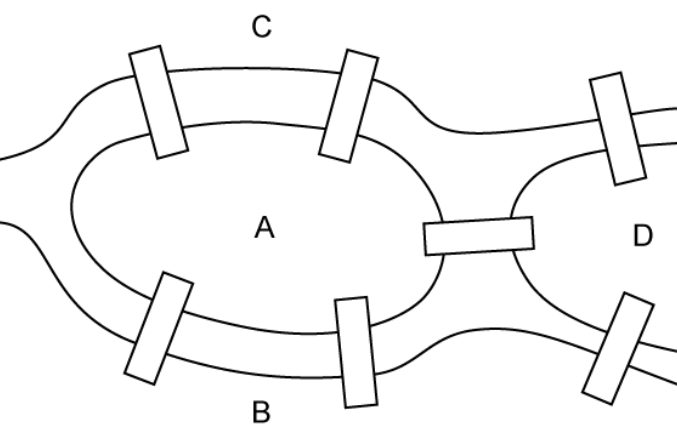
\includegraphics[width=0.62\textwidth]{imgs/background/euler-bridges-01.png}
    \footnotesize b)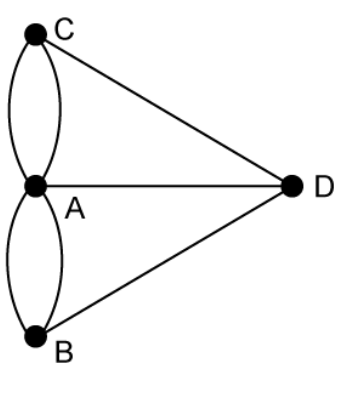
\includegraphics[width=0.32\textwidth]{imgs/background/euler-bridges-03.png}
    \caption{\textit{A schematic representation of the seven bridges of Königsberg problem (fig.a), for which Euler (1707–1783) proposed a negative resolution in his famous 1736 paper, laying the foundation for modern graph theory. The question was if it is possible to traverse all the bridges only once and come back to the point where the trip was started. The answer was negative – it is not possible to get across all bridges exactly once. Mathematically the problem comes down to looking for a Eulerian cycle in a multigraph (multiple edges connecting two vertices) with four nodes and seven edges (fig.b).}}
    \label{fig:bg.gnn.konigsbridge}
\end{figure}
The theory of graphs (also graph theory) can be traced back at least to the illustrious swiss mathematician Leonhard Euler, who in a 1736 paper \mycite{gazette_1987} solved a puzzle about an optimal tour of the town of Königsberg (\cref{fig:bg.gnn.konigsbridge}). Some more developments were made in the $19th$ century, the very term \say{graph} was introduced in this period by Sylvester in a paper published in 1878 in Nature \mycite{Sylvester1878ChemistryAA}, where he draws an analogy between \say{quantic invariants} and \say{co-variants} of algebra and molecular diagrams. The field straight-up exploded during the $20th$ century, the first textbook on graph theory was published in 1936 by Dénes Kőnig, followed by many others \mycite{tutte2001graph}; currently graphs are one of the principal objects of study in discrete mathematics. Graphs, in the realm of mathematics and computer science, are powerful mathematical abstractions used to model relationships between entities. In its basic type, a simple graph G can be defined as the couple:
\begin{equation}
    \label{eq:bg.gnn.graph-def}
    G = (V,E)
\end{equation}
where $V = \{v_1,v_2,...,v_N\}$ is the set of \textit{vertices} or \textit{nodes}, the entities ($n = |V|$), and $E = \{(v_i,v_j) | v_i,v_j \in V; i \ne j\}$ is the set of \textit{edges} ($m = |E|$), also called links, modeling the relationship between two entities. A basic distinction is made between \textit{undirected} graphs, where edges link two vertices symmetrically, i.e. there is no difference between the edges $(v_i,v_j)$ and $(v_j,v_i)$; and \textit{directed} graphs, where edges link two vertices asymmetrically, thus $(v_i,v_j)$ and $(v_j,v_i)$ would be two separated edges \mycite{cormen2022introduction}. Moreover two other categorization are generally made: considering the types of its components and their behavior  over time. 
A graph can be \textit{homogeneous}, when nodes and edges of the graph have all the same type; or \textit{heterogeneous} when nodes and edges are associated with different types. More specifically, in a heterogeneous graph $(V, E, \phi, \psi)$, each node $v_i$ is associated with a type $\phi(vi)$ and each edge $e_j$ with a type $\psi(ej)$. 
When input features or the topology of the graph vary with time, i.e. the existence of nodes and edges may change at different points in time, the graph is regarded as \textit{dynamic}, otherwise is considered \textit{static}. The time information should be carefully considered in dynamic graphs \mycite{zhou2021graph,wang2021mthetgnn}. Note that these categories are orthogonal, meaning that these properties can be combined in the same graph, e.g. one can deal with a dynamic directed heterogeneous graph.
%%% cyclic/acyclic graph

%%% immaginie di applicazione grafi in real world
One of the typical application of graphs is modeling the relationships inside social networks \mycite{Wu_Lian_Xu_Wu_Chen_2020}, tools to study patterns in collective behaviour of people, institutions and organizations, where the set of social actors can be represented with the nodes of the graph, and their relative interactions are represented by the edges (e.g. the standard example for a social graph would be a “friendship graph”; here, $V$ is again a set of people and $E$ is the set of $(u, v) \in V$ such that $u$ and $v$ are friends). This perspective on social network provides a set of methods for analyzing the structure of whole social entities as well as a variety of theories explaining the dynamics and patterns observed in these structures \mycite{wasserman_faust_1994}. Even though realities such as social networks can be easily seen as graphs and modeled accordingly this data structures are an extremely powerful and general representation of data, many other domains can actually be modeled as graphs, like images and text. Although counterintuitive, one can learn more about the symmetries and structure of images and text by viewing them as graphs. 
Traditionally, we visualize images as rectangular grids with image channels, often representing them as arrays. However, an alternative way could be seeing images as graphs possessing a regular structure, where each pixel is a node connected to each neighboring pixels through an edge (\cref{fig:bg.graph_smile}). Specifically, each non-border pixel will maintain precisely 8 neighbors, and the information stored at every node could be a 3-dimensional vector signifying the RGB value of the corresponding pixel. Also text can be easily converted into a graph format by assigning numerical indices to individual characters, words, or tokens, thus creating a sequence of these indices to represent the text. This process yields a straightforward directed graph, where each word or token is a node connected to the succeeding node through an edge. Of course, this is not usually how text and images are encoded: these graph representations are redundant since all images and all text will have very regular structures. In practice, images have a banded structure in their adjacency matrix because all nodes (pixels) are connected in a grid; and the adjacency matrix for text is just a diagonal line, because each word only connects to the prior word, and to the next one, but those trivial examples are supposed to serve as an intuition of how flexible graphs are and how wide can thus be the range of their applications \mycite{distilPub-sanchez-lengeling2021a}.

%%% more detailed examples
\begin{figure}
    \centering
    \footnotesize a)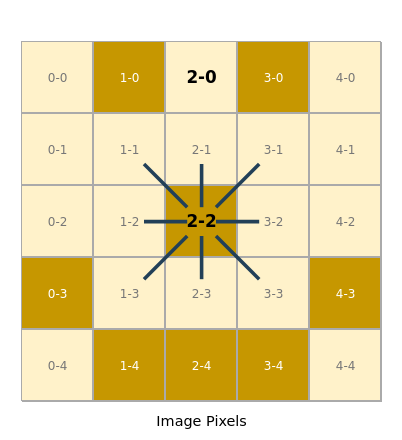
\includegraphics[width=0.3\textwidth]{imgs/background/smile-graph-01.png}
    \footnotesize b)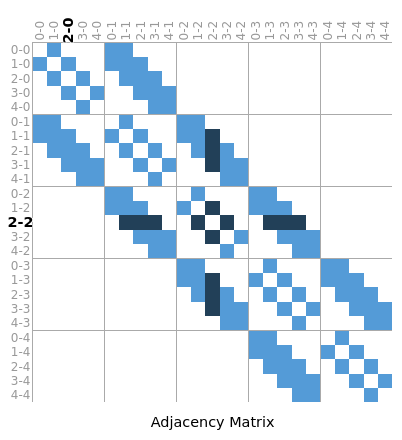
\includegraphics[width=0.3\textwidth]{imgs/background/smile-graph-02.png}
    \footnotesize c)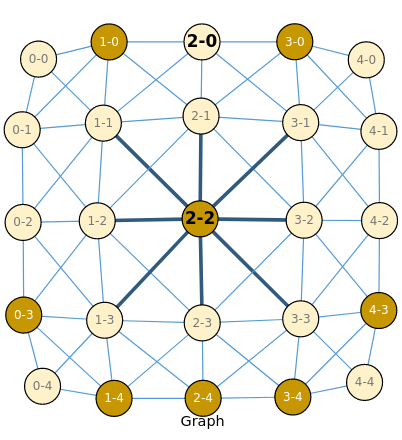
\includegraphics[width=0.3\textwidth]{imgs/background/smile-graph-03.png}
    \caption{\textit{A way of visualizing the connectivity of a graph is through its adjacency matrix. Picture a) shows a simple $5\times5$ image of a smiley face and each of the 25 pixels is indexed as the elements of a $5\times5$ matrix. In picture b) we can see the one of the possible adjacency matrices representing the graph of our smiley face image. This matrix has dimension $n_{nodes}\times n_{nodes}$ ($25\times25$), given that each pixel is a node, connected to all its neighboring pixels through an edge (fig.a,b,c highlights pixel 2-2). Rightmost picture (fig.c), shows the actual graph encoding the smiley image. It is important noticing that each of these three representations below are different views of the very same piece of data \mycite{distilPub-sanchez-lengeling2021a}.}}
    \label{fig:bg.graph_smile}
\end{figure}


%%% graph representation, adjacency list/mat ecc...
\subsubsection{Graph representation}
\label{sec:bg.gnn.graph-repr}
Before going into the details of machine learning applied to graphs, we propose here an introduction on how to represent graphs, their components and the relative features. This problem is crucial to encode real world information into graph models and to be able to exploit the complete potentiality of such abstractions in real world applications. Machine learning models typically take rectangular or grid-like arrays as input, more generally we talk about tensors. In mathematics, a tensor is an algebraic object that describes a multilinear relationship between sets of algebraic objects related to a vector space. Tensors may map between different objects such as vectors, scalars, and even other tensors \mycite{Vasilescu2009AM}. In machine learning, tensors have a broader definition and usually refers also to multidimensional arrays, often called informally \say{data tensors}. The rationale behind this representation is that data stored in such a format can be readily fed into any artificial intelligence model based on neural networks, thereby opening up the possibility of analyzing them through a diverse range of algorithms and models. So, it’s not immediately intuitive how to represent graph structured data in a format that is compatible with deep learning.

Graphs can have up to four types of elements that can be potentially useful to perform machine learning tasks: nodes, edges and connectivity. A solution to represent the first two is relatively straightforward. The most common choice to represent nodes is to assign to each node $v$ an index $i$ (e.g. an integer) as an identifier, and a $d$-dimensional vector to encode the node features, so that, in general, we will have a node feature matrix $X$ of dimension ${N \times d}$ grouping all node data. For what concerns edges we can simply follow the definition (\cref{sec:bg.gnn.graph-base}) identifying each edge $e$ by the couple of nodes it connects in the graph (e.g. if edge $e$ connect nodes $i$ and $j$, we have $e = (v_i,v_j)$) and follow the same idea, if necessary, to encode edge features (in this case the edge feature matrix will have dimension $M \times d$, being $M$ the number of edges) \mycite{cormen2022introduction}. However, representing a graph’s connectivity is more complicated. Several data structures have been proposed to tackle this problem, among them three have resulted to be the most efficient and thus the most used in practice: adjacency matrix, incidence matrix and adjacency list.

%\begin{figure}
%    \label{fig:bg.graph_repr}
%    \centering
%    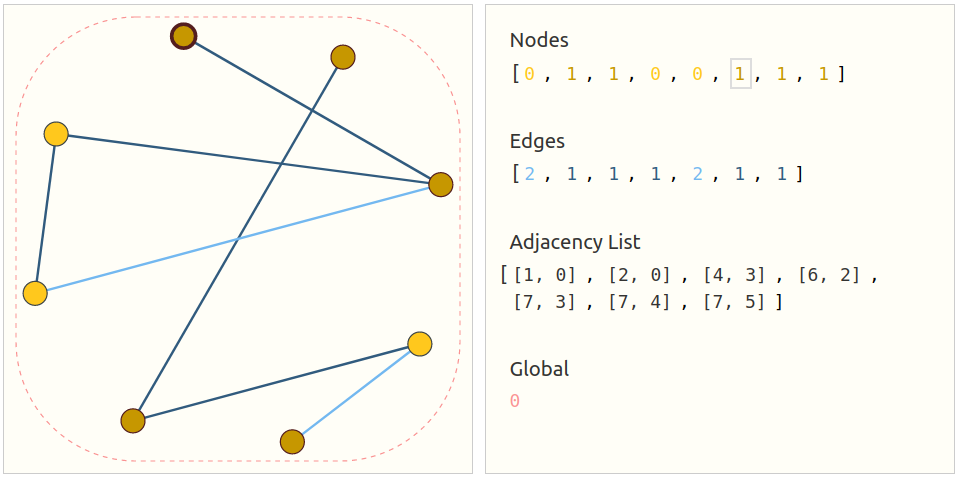
\includegraphics[width=\textwidth]{imgs/background/graph-repr.png}   
%    \caption{\textit{Notice that the figure uses scalar values per node/edge/global features, but most practical representations can have vectors/tensors to encode features per graph attribute. Instead of a node feature tensor of size $N = |\mathcal{V}|$ we will be dealing with node tensors of size $[N,d]$ (where $d$ is the dimension of the node features). Same reasoning holds for the other graph attributes.}}
%\end{figure}

The \textit{adjacency matrix} is a two-dimensional tensor ($n \times n$, being $n$ the number of nodes), in which the rows represent source vertices and columns represent destination vertices. Data on edges and vertices must be stored externally. Only the cost for one edge can be stored between each pair of vertices. We note that any two vertices connected by an edges are called adjacent, thus the term \textit{adjacency}. The \textit{incidence matrix} is a two-dimensional tensor ($n \times m$, being $m = |E|$ the number of edges), in which the rows represent the vertices and columns represent the edges, so that the entries indicate the incidence relation between the vertex at a row and edge at a column (an edge $e$ is said to be incident to a node $v$, if $e$ is connected to $v$). \textit{Adjacency lists} can be of two types. In one case nodes can be stored as records or objects, and every vertex stores the list of its adjacent vertices. This data structure allows the storage of additional data on the vertices, and even additional data on edges can be stored if they are also stored as objects, in which case each vertex stores its incident edges and each edge stores its incident vertices. The second case is the most common format of \textit{adjacency list}, where all edges are stored together in one single list, which loses the explicit information of the vertices adjacent to a particular node, gaining on efficiency on space usage \mycite{cormen2022introduction}.  

Perhaps, since it can be easily tensorisable the most obvious choice would be to use an adjacency matrix to represent a graph for machine learning purposes. Yet, this particular representation comes with certain limitations. As illustrated by the example dataset table, the quantity of nodes within a real world graph can reach millions, with a highly fluctuating number of edges per node. Consequently, this frequently results in adjacency matrices with significant sparsity, rendering them highly inefficient in terms of space usage. Another big issue is that there can be many adjacency matrices encoding the same connectivity relations (i.e. the same graph), and there could be no guarantee that these different matrices would produce the same result in a deep neural network, that is to say, they are not permutation invariant. The permutation invariance property is a fundamental inductive bias of graph-structured data, resulting in the fact that for a graph with $n$ nodes, there are up to $n!$ different adjacency matrices that are equivalent representations of the same graph. Learning permutation invariant operations is an indipendent area of recent research, we refer the reader to \mycite{mena2018learning,murphy2019janossy} for further details.

There are now dozens (if not hundreds) textbooks available on the subject (\cite{griffin2023applied,cormen2022introduction,diestel2017graph,bondy2011graph,berge1976graphs}; only to cite few relevant ones); we refer the reader to the mentioned books to delve further into the details of all aspects of graph theory given that such a discussion deviates from the main purpose of this background introduction, which is to show the importance of graphs in mathematics, computational sciences and various fields, and why recently a great interest in applying deep learning to these concepts arose. 

%%% ML sui grafi
\subsection{Deep Learning on graphs}
\label{sec:bg.gnn.DL-on-graphs}
Deep learning is part of a broader family of machine learning (ML) methods, mainly based on extracting patterns from raw data using Artificial Neural Networks (ANNs) and representation learning. The adjective \say{deep} in deep learning refers to learning complicated concepts by building them from simpler ones in a hierarchical or multi-layer manner \mycite{LeCun2015DeepL}. Artificial neural networks are popular realizations of such deep multi-layer hierarchies. In the past few years, the growing computational power of modern GPU-based computers and the availability of large training datasets have allowed successfully training neural networks with many layers and degrees of freedom \mycite{Bronstein_2017}.

\subsubsection{history}
\label{sec:bg.gnn.DL-history}
The history of deep learning can be traced back several decades, with its roots in ANNs and machine learning. In 1943, drawing inspiration from the structure of a biological neuron, Warren McCulloch (a neuroscientist) and Walter Pitts (a logician) proposed a mathematical model of an artificial neuron, providing a foundational concept for the birth of artificial neural networks \mycite{mcculloch-pitts-1943}.   

Basically, a neuron in our brain takes an input signal (through the \textit{dendrites}), processes it in its nucleus (\textit{soma}), passes the output through a cable like structure to other connected neurons (\textit{axon} to synapse to another neuron’s dendrites). Although this oversimplification may not align with the biological intricacies of neurons, it offers a high-level representation of how a neuron in our brain functions: receiving input, processing it, and producing an output. This first computational model can be broken down in two parts (\cref{fig:bg.first-neurons}a): the first part, $g$ takes one or more inputs, performs an aggregation and based on the obtained value the second part, $f$ produces an output, i.e. makes a decision. It is following the idea that the interconnection of many simple units, carrying out a simple task, can create the astonishing complexity of human brain that the first artificial neuron was born.

\begin{figure}
    \footnotesize a)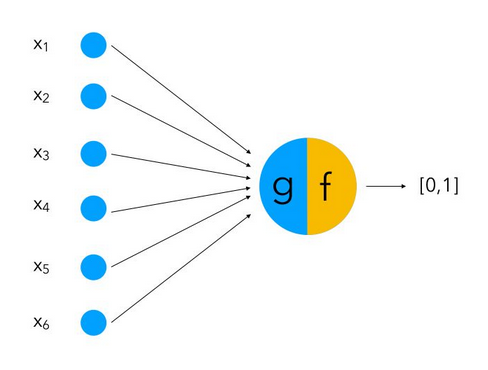
\includegraphics[width=0.45\textwidth]{imgs/background/mcculloch-pitts-02.png} 
    \footnotesize b)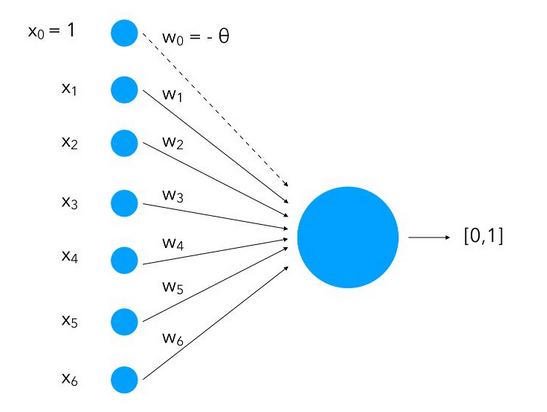
\includegraphics[width=0.45\textwidth]{imgs/background/rosenblatt-02.png} 
    \caption{\textit{On the left (fig.a) a schema of the first artificial neuron introduced by McCulloch and Pitts in 1943. On the right (fig.b) the schema of the perceptron model, introduced by Rosenblatt in 1957. The crucial differences introduced by Rosenblatt are that a weight ($w_i$) is attached to each input and an input ($x_0$) of value $1$ and weight $-\theta$ is added (this is called bias). Instead of having only the inputs and the weight and compare them to a threshold, the perceptron also learn the threshold as a weight for a standard input of value $1$. This produces sort of a weighted sum of inputs, to which we apply an activation function, resulting in the final output.}}
    \label{fig:bg.first-neurons}
\end{figure}
Later on, in 1957, Frank Rosenblatt developed the perceptron, a single-layer neural network capable of binary classification \mycite{rosenblatt-1958-perceptron}.  It was designed to overcome most issues of the McCulloch-Pitts neuron: it can process non-boolean inputs and it can assign different weights to each input automatically; the threshold $\Theta$ is computed automatically (\cref{fig:bg.first-neurons}b). It gained attention for its potential in pattern recognition tasks. The version of Perceptron we use nowadays as standard artificial neuron was introduced in 1969 by Minsky and Papert. Their book criticized the limitations of perceptrons and brought a major improvement to the previous model adding an activation function after the in put aggregation step. The activation function might take several forms and should restrict the weighted sum into a smaller set of possible values that allows a better classification of the output \cite{minsky-papert-1969-perceptrons}. It’s a smoother version than the thresholding applied before. The first comprehensive learning algorithm for supervised, deep, feedforward, multilayer perceptrons was introduced in 1967 by Alexey Ivakhnenko and Lapa \mycite{Ivakhnenko1967CyberneticsAF}.  In a subsequent 1971 paper, they described a deep network with eight layers trained by the group method of data handling. 

In 1989, the book \say{Parallel Distributed Processing} by Rumelhart, Hinton, and Williams popularized the backpropagation algorithm reviving the interest in the possibility of an efficient training for deep neural networks, and posed the basis for all modern neural network based ML algorithms \mycite{rumelhart-hinton-1989}. One of the first big result that draw attention to deep networks was AlexNet \mycite{krizhevsky2012-nips}, a deep Convolutional Neural Network (CNN) developed by Alex Krizhevsky, that won the ImageNet competition, marking a significant breakthrough and initiating a surge of interest in deep learning. AlexNet competed in the ILSVRC \mycite{ILSVRC15} on September 30, 2012. The deep network achieved a top-5 error of $15.3\%$, more than $10.8$ percentage points lower than that of the runner up. 

In recent years, since the growing availability of GPU processing, deep neural networks have been able to achieve outstanding results in many areas related to Machine Learning. In 2014 Ian Goodfellow introduced Generative Adversarial Networks (GANs), a powerful tool for deep generation of data \mycite{goodfellow2014-GANs}; in the same year DL also made strides in reinforcement learning (a sub-field of ML), with models like Deep Q Networks (DQN) \mycite{Mnih2015-HumanlevelCT}, showing more of the potentiality of deep networks with respect to shallow ones. Another important step forward was made with the introduction of the Transformer architecture, in the 2017 paper \say{Attention is All You Need} \mycite{vaswani2017-attention} revolutionized natural language processing (NLP), the interdisciplinary sub-field of computer science and linguistics primarily concerned with giving computers the ability to support and manipulate natural language and speech. This led to an important breakthrough in NLP, and in the whole AI spectrum, when the language model BERT (Bidirectional Encoder Representations from Transformers) came out. Being one of the first language model based on trasformers, BERT achieved state-of-the-art results in various NLP tasks thanks to the fact that its the pre-trained model can be fine-tuned with just one additional output layer to create state-of-the-art models for a wide range of applications, such as question answering and language inference, without substantial task-specific architecture modifications.  \mycite{devlin2018-bert}.


\subsubsection{Geometric Deep Learning}
\label{sec:bg.gnn.geo-deep-learning}
For almost two thousand years the word geometry has been a synonym of Euclidean geometry, until this hegemony was disrupted, during the nineteenth century, when Lobachevsky, Bolyai, Gauss, and Riemann independently constructed instances of non-Euclidean geometries, signaling the end of Euclid's monopoly \mycite{coxeter1998-non-euclidean-geom}. As that century concluded, these inquiries had fragmented into distinct domains. Mathematicians and philosophers engaged in debates regarding the authenticity and interconnections of these geometries, alongside discussions on the essence of the \say{one true geometry}. A wide array of neural network architectures tailored for diverse data types exists, yet few overarching principles tie them together. As in the past, this lack of cohesion complicates comprehension regarding the interplay among different methodologies, consequently leading to redundant rediscovery and re-branding of identical concepts across distinct application domains. For anyone who is a novice trying to learn the field, absorbing the sheer volume of redundant ideas can be a true nightmare \mycite{bronstein2021geometric}.

Geometric Deep Learning (GDL) was born as a \say{geometrisation} attempt, with the mindset of bringing order into the chaos of deep learning, obtaining a systematisation of this field. THe key of this approach is to derive different inductive biases and network architectures implementing them from first principles of symmetry and invariance. GDL is thus an umbrella term for emerging techniques attempting to extend (structured) deep neural models to non-Euclidean spaces, such as graphs and manifolds. Deep learning models have excelled notably in handling signal-based data like speech, images, or video, where an inherent Euclidean structure is present. However, in recent years, there has been an increasing fascination with the endeavor to employ learning approaches for non-Euclidean geometric data, given that such kinds of data arise in numerous real-life applications like social networks and many others (see \cref{sec:bg.gnn.graph-base} for more examples).

In this section on GDL we propose an overview of prevalent deep learning architectures, even though we acknowledge the continuous emergence of new neural network variants on a daily basis. Therefore, the objective is not to provide an exhaustive coverage of every potential architecture, but we aspire for the forthcoming sections to be sufficiently illustrative. The most common deep learning architectures are thus shown here by utilizing the perspective of invariances and symmetries, that can be a useful lens for an easy categorization of any future GDL developments. There are mainly three kind of architectures that cover the geometric data domains: Convolutional Neural Networks (CNNs), group-equivariant CNNs, and Graph Neural Networks (GNNs). 

%According to a popular belief, the Erlangen Programme was delivered in Klein’s inaugural address in October 1872. Klein indeed gave such a talk (though on December 7 of the same year), but it was for a non-mathematical audience and concerned primarily his ideas of mathematical education. What is now called the ‘Erlangen Programme’ was actually a research prospectus brochure \textit{Vergleichende Betrachtungen über neuere geometrische Forschungen} (“A comparative review of recent researches in geometry”) he prepared as part of his professor appointment. See Tobies (2019).

\paragraph{Convolutional Neural Networks}
\label{sec:bg.gnn.cnn}
\begin{figure}[t]
    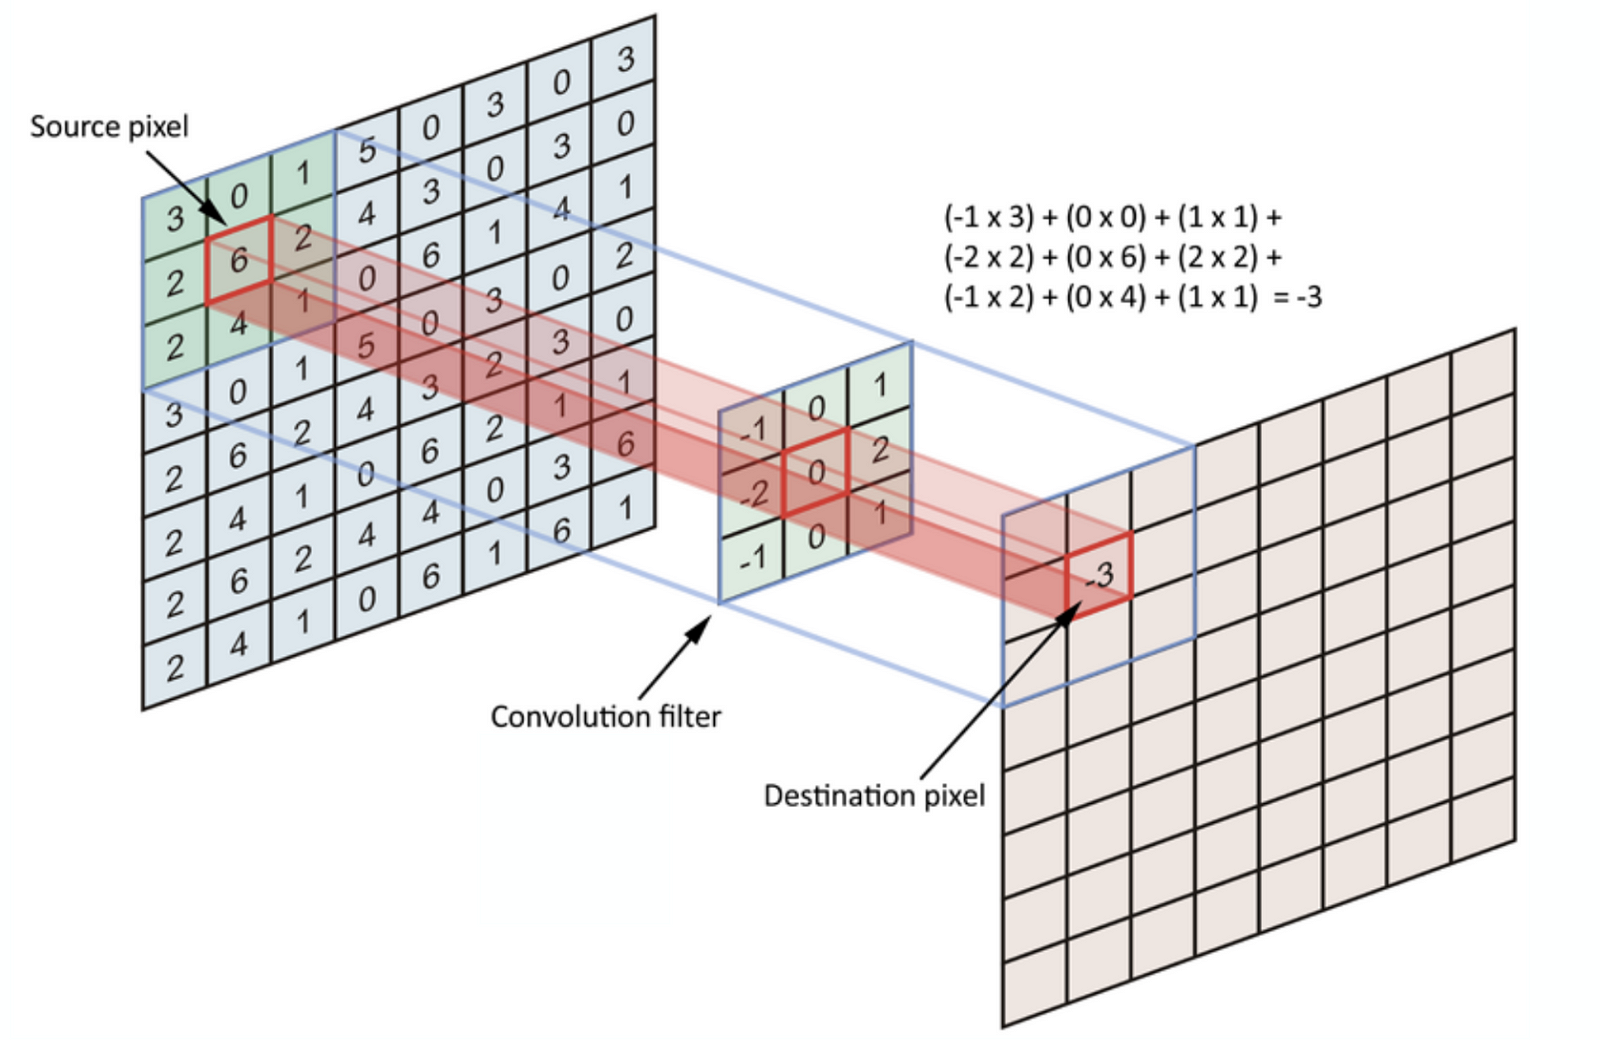
\includegraphics[width=\textwidth]{imgs/background/convolution_op.png}
    \caption{\textit{The process of convolution on an input image ($8 \times 8$), assuming each pixel has an integer $p$ as value ($p \in \{0,1\}$). In this $2$-dimensional case the filter (or kernel) is a 2D matrix ($3\times3$). In the convolution operation the kernel is strided on the input signal to compute each destination pixel of the output. The actual mathematical convolution is done by computing the dot-product between the kernel and a region of the same dimension of the input image, moving the filter all over the input to obtain each of the output components.}}
    \label{fig:bg.convolution}
\end{figure}
CNNs are perhaps the earliest, and currently among the most successful, deep learning architectures in a variety of tasks, in particular, in computer vision. They are also known as shift invariant or space invariant artificial neural networks (SIANN, \cite{chaman2021-siann}), based on their shared-weights architecture and translation invariance characteristics. CNN have a broad range of applications such as in image and video recognition \mycite{valueva2020-cnn-application}, recommender systems \mycite{dieleman2013-cnn-recommendation}, medical image analysis \mycite{yu2021-cnn-medical}, and also natural language processing \mycite{collobert2008-cnn-nlp}, in the beginning of this field. A typical CNN used in computer vision applications consists of multiple convolutional layers, passing the input image through a set of filters followed by point-wise non-linearity $\xi$ (typically, half-rectifiers $\xi(z) = max(0, z)$ or ReLU \mycite{nairHinton2010-relu} are used, although practitioners have experimented with a diverse range of choices for the activation function), and additional layers, including pooling layers, fully connected layers, and normalization layers.

The convolutional layer is the core building block of a CNN, it is defined by its parameters, primarily a collection of learnable filters (or kernels) that possess a relatively small receptive field but span the entire depth of the input volume. During the forward pass, each filter is \say{convolved} across the width and height of the input volume, computing the dot product between the filter entries and the input, producing a (when dealing with images, 2-dimensional) activation map of that filter (\cref{fig:bg.convolution}). Consequently, the network learns filters that trigger upon detecting certain distinctive features at specific spatial positions within the input. Following this, the feature map obtain after the convolution operation can be used as input to another layer of the same type (but with a different kernel) or it can be fed to pooling, to reduce the dimensions of data by combining the outputs of neuron clusters at one layer into a single neuron in the next layer, and/or normalization layers. The combination of convolution, pooling and/or normalization is so common in CNN architectures, that the last two can be considered as a building component of a fully-functioning convolutional layer \mycite{LeCun2015DeepL}. After one or many convolutional steps, in a typical CNN, there are some fully connected layers arranged in a multi-layer perceptron (MLP) fashion, that aim to classify the encoded deep representation of the input data obtained with the convolution.



\paragraph{Group equivariant CNN}
\label{sec:bg.gnn.geCNN}
\cite{taco2016-geCNN} showed that it is possible generalise the convolution operation from signals on a Euclidean space to signals on any homogeneous space $\Omega$ acted upon by a group $\mathrm{G}$, i.e. convolutional networks can be generalized to exploit larger groups of symmetries, including rotations and reflections. By analogy to the Euclidean convolution where a translated filter is matched with the signal, the idea of group convolution is to move the filter around the domain using the group action, e.g. by rotating and translating. By virtue of the transitivity of the group action, we can move the filter to any position on $\Omega$.

Convolutional layers are highly efficient within a deep network due to the translation equivariance present in all its layers. This property implies that shifting an image and subsequently passing it through a series of layers is equivalent to initially processing the original image through the same layers and then shifting the resulting feature maps (while considering edge-effects). Essentially, each layer maintains the symmetry of translation, enabling its utilization not only in the initial layers but also in the higher layers of the network. The key concept behind Group-equivariant CNNs (G-CNN) is that convolutional networks can be generalized to exploit larger groups of symmetries, including rotations and reflections. This signifies that within the representation space, every vector possesses an associated pose that can be altered by the elements within a specific transformation group, denoted as G. This supplementary structure enhances our ability to model data with greater efficiency. In a G-CNN, a filter identifies co-occurrences of features exhibiting the desired relative pose and can recognize such a feature configuration in any global pose using an operation known as the G-convolution. For further details on this type of deep networks we suggest the following material, the already cited \mycite{taco2016-geCNN} and \mycite{bronstein2021geometric}.



\paragraph{Representation Learning}
\label{sec:bg.gnn.repr-learning}
Representation Learning, which is the task of learning representations for complex structured data, is quite challenging with non-euclidean ones. In the last decade, many successful models have been developed for certain kinds of structured data, including data defined on a discretized Euclidean domain. For instance, sequential data, such as text or videos, can be modelled via recurrent neural networks \mycite{TEAlab2018334}, which can capture sequential information, yielding efficient representations as measured on machine translation and speech recognition tasks. Another example are Convolutional Neural Networks (CNNs)\mycite{Lecun1998cnn} have been successfully applied to tackle problems such as image classification (\cite{venkatesan2017convolutional}), semantic segmentation (\cite{jégou2017layers}) or machine translation (\cite{gehring2017convolutional}), where the underlying data representation has a grid-like structure. These architectures efficiently reuse their local filters, with learnable parameters, by applying them to all the input positions \mycite{LeCun2015DeepL}. However these major successes have been restricted to particular types of data that have a simple relational structure (e.g. sequential data, or data following regular patterns), many interesting tasks involve data that can not be represented in a grid-like structure and that instead lies in an irregular domain. This is the case of a large number of systems across various areas including natural science (physical systems (\cite{pmlr-v80-sanchez-gonzalez18a}), social science (social networks as in the example in \cref{sec:bg.gnn.graph-base}), protein-protein interaction networks (\cite{nips2017_PPI}), knowledge graphs (\cite{ijcai2017p250}) and many other research areas (\cite{nips2017_combOpt}), to name a few. Such data can usually be represented in the form of graphs \mycite{veličković2018gat}.

%Machine learning with graphs blends the line between this distinction because of two key differences in approaching the problem.

\subsection{GNNs}
\label{sec:bg.gnn.gnns}
Graph Neural Networks (GNNs) have been introduced in \mycite{Gori2005graphDomain,gnnModel2009} as a generalization of recursive neural networks that can directly deal with the more general class of graphs and their impressive performance has propelled these deep learning models to the forefront of widely utilized methods in graph analysis today. The fundamental principle behind GNNs is to produce representations of graph (and/or its components) that can be used in downstream tasks such as graph or node classification. GNNs are among the most general class of deep learning architectures currently in existence, and it is a fact, most other deep learning architectures can be understood as a special case of the GNN with additional geometric structure. It is important to remind the reader that GNNs are not the exclusive tools for modeling graph-structured data; for example graph kernels \mycite{vishwanathan2010-graph-kernels} and random-walk methods \mycite{grover2016-node2vec,perozzi2014-deepwalk} were previously among the most prevalent. However, in current times, GNNs have predominantly supplanted these approaches due to their inherent adaptability, allowing for superior modeling of the underlying systems.

The first motivation of GNNs is rooted in the long-standing history of neural networks for graphs. In the nineties, Recursive Neural Networks are first utilized on directed acyclic graphs (\cite{Sperduti1997,Frasconi1998}). Afterwards, Recurrent Neural Networks and Feedforward Neural Networks are introduced into this literature respectively in (\cite{gnnModel2009}) and (\cite{Micheli2009}) to tackle cycles. Although being successful, the universal idea behind these methods is building state transition systems on graphs and iterate until convergence, which constrained the extendability and representation ability. Recent advancement of deep neural networks, especially convolutional neural networks (CNNs) resulted in the rediscovery of GNNs. 

A Graph Neural Network (GNN) is a transformation that can be optimized across all attributes of a graph, including nodes, edges, and global-context, while preserving the symmetries of the graph (permutation invariances). In this section a basic approach to constructing GNNs is introduced, fllowing the \say{message passing neural network} framework as proposed in (\cite{gilmer2017-message-passing}), and employing the architectural schematics of Graph Nets introduced by (\cite{battaglia2018-relational}). GNNs follow a "graph-in, graph-out" architecture, meaning they take a graph as input, with information embedded in its nodes, edges, and global-context. They then progressively enrich these embeddings without altering the connectivity of the initial graph.

%This first step of GNN design, usually called Graph Representation Learning (GRL) aim at learning low-dimensional continuous vector representations for graph-structured data, also called embeddings. Broadly speaking, GRL can be divided into two classes of learning problems, unsupervised and supervised (or semi-supervised) GRL. The first family aims at learning low-dimensional Euclidean representations that preserve the structure of an input graph. The second family also learns low-dimensional Euclidean representations but for a specific downstream prediction task such as node or graph classification. Different from the unsupervised setting where inputs are usually graph structures, in supervised settings inputs are usually composed of different signals defined on graphs, commonly known as node or edge features.

%GNNs consist of an iterative process, which propagates the node states until equilibrium; followed by a neural network, which produces an output for each node based on its state. This idea was adopted and improved by Li et al. (2016), which propose to use gated recurrent units (Cho et al., 2014) in the propagation step.

Having introduced the basic concepts around graphs, to better better comprehend their success we present an overview of the principal tasks that can be performed through graph representation. As a unique non-Euclidean data structure for machine learning, graph analysis focuses on tasks such as graph classification, node classification, link prediction, and clustering. Despite this variety, there are three general types:
\begin{itemize}
    \item \textbf{Graph-level} In a graph-level task, our goal is to predict the property of an entire graph. For instance, when dealing with a molecular representation structured as a graph, a common objective could be predicting the fragrance of the molecule or its likelihood to bind to a receptor associated with a particular disease. This can be likened to image classification tasks like MNIST \mycite{lecun1998-mnist} and CIFAR \mycite{cifair10}, where the goal is to assign a label to an entire image. In the realm of text analysis, a comparable task is sentiment analysis, where the aim is to determine the overall mood or emotion of an entire sentence in one go.
    
    \item \textbf{Node-level} For a node-level task, we predict some property for each node in a graph. An example could be a GNN used for a node prediction task on the Cora dataset (\cite{mcCallum2000-cora}) to predict the subject of a paper given its words and citations network. The Cora dataset consists of 2708 scientific publications classified into one of seven classes, resulting in a citation network composed of 5429 links. Each article in the network is represented by a node, that can be classified into one of the seven classes availble (i.e. the subjects of the each paper).
    
    \item \textbf{Edge-level} For an edge-level task, we want to predict the property or presence of edges in a graph. An instance of edge-level inference can be observed in image scene comprehension (\cref{fig:bg.gnn.scene-under}). Beyond merely recognizing objects within an image, deep learning models can also forecast the associations between these objects. This can be framed as edge-level classification: given nodes representing the image's objects, our goal is to anticipate which nodes are linked by an edge and determine the value of that edge. If our objective is to uncover relationships between entities, we might envision the graph as fully interconnected. From there, we can prune edges based on their predicted values to derive a sparser graph that highlights meaningful connections.
\end{itemize}

\begin{figure}
    \centering
    \footnotesize a) 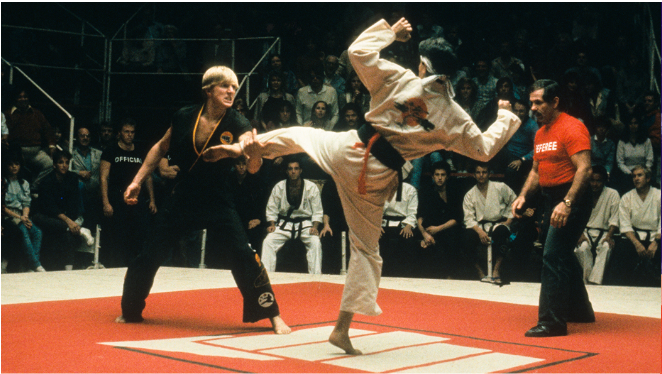
\includegraphics[width=0.46\textwidth]{imgs/background/scene-under-01.png}
    \footnotesize b) 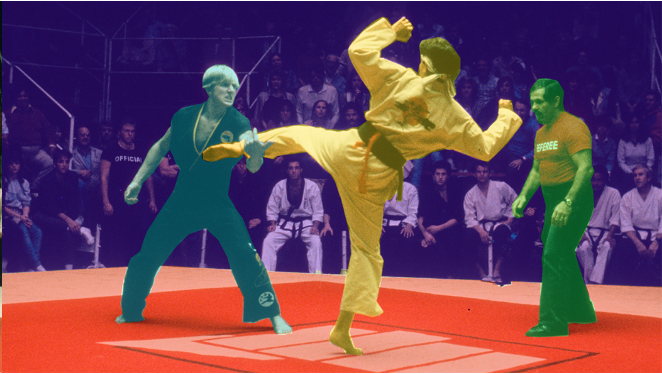
\includegraphics[width=0.46\textwidth]{imgs/background/scene-under-02.png}
    \footnotesize c) 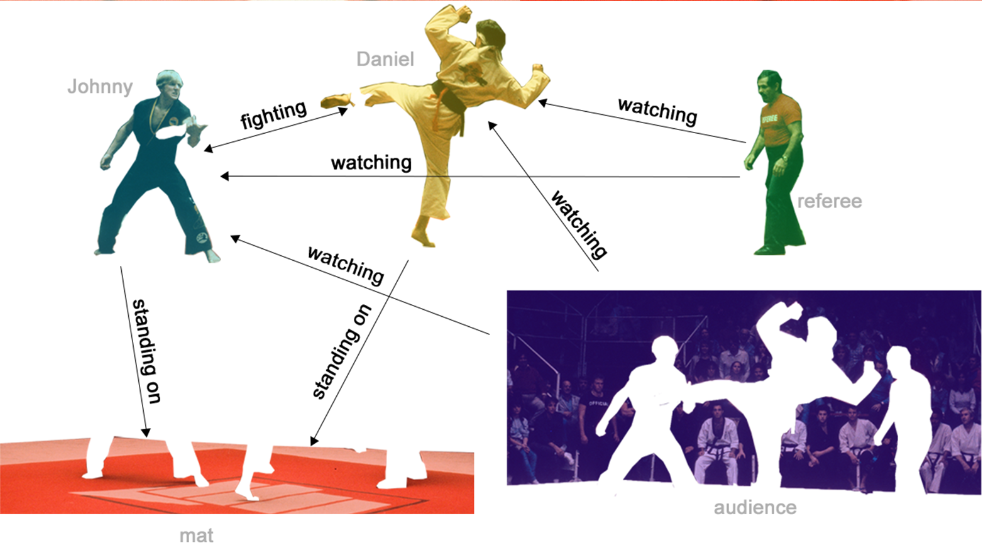
\includegraphics[width=0.8\textwidth]{imgs/background/scene-under-03.png}
    \caption{\textit{An example of a scene understanding task. In (fig.b), above, the original image (fig.a) has been segmented into five entities: each of the fighters, the referee, the audience and the mat. (fig.c) shows the relationships between these entities as edges of a graph connecting the elements (nodes) in the scene. Note that in this example the extracted representation is a directed-graph with three edges attributes, the actions performed by the entities in the scene (fighting, watching, standing on).}}
    \label{fig:bg.gnn.scene-under}
\end{figure}

The three levels of prediction problems described above (graph-level, node-level, and edge-level), can be solved with the Graph Neural Network model class. 

%%%% TODO: poolong section
\subsubsection{Pooling}
\label{sec:bg.gnn.graph-pooling}
The following example are going to implicitly focus on binary classification, although this framework can be seamlessly expanded to handle multi-class or regression scenarios. When the objective is binary prediction for nodes and the graph already includes node information, the process is uncomplicated: for each node embedding, utilize a linear classifier \mycite{daigavane2021-conv-on-graphs}. 

However, it is not always so simple. For instance, you might have information in the graph stored in edges, but no information in nodes, but still need to make predictions on nodes. We need a way to collect information from edges and give them to nodes for prediction. We can do this by pooling. Pooling proceeds in two steps: First for each item to be pooled, gather each of their embeddings and concatenate them into a matrix; second the gathered embeddings are then aggregated, usually via a sum operation. If we only have node-level features, and need to predict a binary global property, we need to gather all available node information together and aggregate them. This is similar to Global Average Pooling layers in CNNs. The same can be done for edges. Having successfully showcased the creation of a basic GNN model and its ability to make binary predictions by transmitting information between various graph segments, this pooling technique should be kepth in mind as a fundamental component for crafting more advanced GNN models.

%%%% TODO: message passing
\subsubsection{Message Passing}
\label{sec:bg.gnn.message-passing}
We could make more sophisticated predictions by using pooling within the GNN layer, in order to make our learned embeddings aware of graph connectivity. We can do this using message passing, where neighboring nodes or edges exchange information and influence each other’s updated embeddings \mycite{gilmer2017-message-passing}.

Message-passing on GNNs operates through a three-step process: \textit{i}) for every node within the graph, it collects all the embeddings from neighboring nodes; \textit{ii}) it aggregates all these messages, typically using a function like summation; \textit{iii}) the combined messages are then passed through an update function, typically implemented as a learned neural network. Just as pooling can be applied to either nodes or edges, message passing can occur between either nodes or edges. When executed in a single iteration, this sequence of operations contitutes the most basic form of a message-passing GNN layer.

This bears a resemblance to a standard convolution in CNNs (\cref{fig:bg.convolution}): fundamentally, both message passing and convolution involve the aggregation and processing of information from neighboring elements to update the value of the element. In the context of graphs, this element is a node, while in images, it corresponds to a pixel. Nonetheless, it's worth noting that the number of neighboring nodes in a graph can vary, unlike in an image where each pixel has a fixed number of neighboring elements. The key achievement of this formulation is that stacking multiple message-passing GNN layers consecutively, a node can eventually assimilate information from the entire graph. At every step, the resulting representation of a node in the graph is influenced by the its neighbors, i.e. the nodes at one-edge distance. This progressively results in gathering information from nodes one-edge further at each layer of the GNN (i.e. each message-passing iteration), so that after three layers, a node has information about the nodes three hops (edges) away from it. It is trivial to notice that with a sufficient number of iteration, this mechanism will cover the whole graph, making the embedding of a node aware of the entire topology of the graph.

%%% TODO: more formal and mathematic definition from MATE paper


\subsubsection{GNNs architectures}
\label{sec:bg.gnn.gnn-archs}
The design and study of GNN layers is one of the most active areas of deep learning at the time of writing, making it a landscape that is challenging to navigate. Fortunately, we find that the vast majority of the literature may be derived from only three “flavours” of GNN layers \mycite{bronstein2021geometric}, which we will present here.

In all three flavours, permutation invariance is ensured by aggregating features from $X_{N_u}$ (potentially transformed, by means of some function $\psi$) with some permutation-invariant function $\oplus$, and then updating the features of node $u$, by means of some function function $\phi$. Typically, $\phi$ and $\psi$ are the learnable, features; with e.g. whereas $\oplus$ is realised as a non-parametric operation such as recurrent neural networks (\cite{murphy2019janossy}). These flavours govern the extent to which $\phi$ transforms the neighbourhood features, allowing for varying degrees of complexity when modelling interactions across the graph.

\paragraph{Convolutional flavour}
\label{sec:bg.gnn.gcn}
In the convolutional flavour (\cite{kipf2016-semisupervised,defferrard2017-convolutional,wu2019-simplifying}), the features of the neighbourhood nodes are directly aggregated with fixed weights
\begin{equation}
    h_u = \phi \left( X_u, \bigoplus_{v \in N_u} C_{uv} \psi(X_v) \right)
\end{equation}
Here, $C_{uv}$ specifies the importance of node $v$ to node $u$’s representation. It is a constant that often directly depends on the entries in $A$ representing the structure of the graph. Note that when the aggregator operator $\oplus$ is chose to be the summation, it can be considered as linear diffusion of position-dependent linear filtering, a generalization of convolution. Even though most of the GNNs used in practice are based on convolution (and thus graph convolutional networks, GCNs), this definition covers most of such approaches, in the sense of commuting with the graph structure, but not all of them.

\paragraph{Attentional falvour}
\label{sec:bg.gnn.gat}
The attentional approach to GNNs is one of the most recent and most interensting. Attention mechanisms have become really popular, almost a \textit{de facto} standard, in many sequence-based tasks (Bahdanau et al., 2015; Gehring et al., 2016). The key advantage that attention mechanisms offer is handling inputs with varying sizes, focusing on the most relevant parts of the input to facilitate informed decision-making.
The attentional \say{flavour} is characterized by implict interactions (\cite{veličković2018gat,monti2016-geometric-mixture,zhang2018-gaan}),
\begin{equation}
    h_u = \phi \left( X_u, \bigoplus_{v \in N_u} a(X_u,X_v) \psi(X_v) \right)
\end{equation}

Here, a is a learnable self-attention mechanism that computes the importance coefficients $\alpha_{uv} = a(X_u, X_v)$ implicitly. They are often softmax-normalised across all neighbors. When $\oplus$ is the summation, the aggregation is still a combination of the neighborhood features, but now the weights are feature-dependent.

\paragraph{Message-passing flavour}
\label{sec:bg.gnn.mp-arch}
Finally, another really common approach to GNNs, the message-passing \say{flavour} (\cite{gilmer2017-message-passing,battaglia2018-relational}) amounts to computing arbitrary vectors (\say{messages}) between adjacent nodes across the edges connecting them, simulating an exchange of information between the graph components,
\begin{equation}
    h_u = \phi \left( X_u, \bigoplus_{v \in N_u} \psi(X_u,X_v) \right)
\end{equation}

Here, $\psi$ is a learnable message function, computing $v$’s vector sent to $u$, and the aggregation can be considered as a form of message passing on the graph. One important thing to note is a representational containment between these approaches: \textit{convolution} $\subseteq$ \textit{attention} $\subseteq$ \textit{message-passing}.  Indeed, attentional
GNNs can represent convolutional GNNs by an attention mechanism implemented as a look-up table $a(X_u, X_v) = C_{uv}$, and both convolutional and attentional GNNs are special cases of message-passing where the messages are only the sender nodes features: $\psi(X_u, X_v) = C_{uv}\psi(X_v)$ for convolutional GNNs and $\psi(X_u, X_v) = a(X_u, X_v)\psi(X_v)$ for attentional GNNs.

%%% GIN, GGNN


\newpage
\section{eXplainable Artificial Intelligence (XAI)}
\label{sec:bg.xai}
Explainable Artificial Intelligence (XAI) stands at the forefront of the evolving field of artificial intelligence (AI) and seeks to bridge the gap between advanced AI models and human comprehension. As AI systems become increasingly sophisticated and pervasive in our lives, understanding their decision-making processes and outcomes is crucial for fostering trust, transparency, and usability. XAI aims to unravel the 'black box' nature of complex AI algorithms, providing insights into how these models arrive at specific conclusions or predictions.

%%% white box - black box

The realm of artificial intelligence (AI) is extensive, intricate, and in a perpetual state of evolution. With the progress in computational capabilities and the ever-expanding pool of data, AI algorithms are being extensively researched and developed for diverse applications, catering to a wide array of potential users and associated risks. Within the AI community, there is a concerted effort to prioritize explainability as a fundamental trait for building trustworthy AI systems. Collaborating with this community, NIST (National Institute of Standards and Technology) has identified additional technical attributes essential for fostering trust in AI \mycite{phillips2021-nist-xai}. In addition to explainability and interpretability, the two big branches of the explaining ML research area, various other characteristics are proposed within AI systems to enhance their trustworthiness. These include accuracy, privacy, reliability, robustness, safety, security (resilience), mitigation of harmful bias, transparency, fairness, and accountability. The interaction of explainability and these AI system attributes may occurs at different stages throughout the AI lifecycle, but this work is focused mainly on the explainability.

NIST identified four main principle, that are significantly shaped by taking into account how the AI system interacts with the human recipient of the information. The specific demands of the situation, the task in progress, and the end-user all play a role in determining the suitable type of explanation for the circumstance. A more precise definitions for three fundamental terms in this definition, \textit{explanation}, \textit{output}, and \textit{process}, should be established before introducing and discussing the principles. An \textit{explanation} refers to the evidence, support, or reasoning associated with a system's output or process. The \textit{output} of a system is defined as either i) the result or ii) the action executed by a machine or system while performing a task. It's important to note that the system's output varies based on the specific task (e.g. for a loan application, the output is a decision: approved or denied; for a movie recommendation system, the output could be a list of recommended movies). The term \textit{process} encompasses the procedures, design, and overall workflow of the system (as referenced in \cite{leslie2021-xai-workbook}). This encompasses the system's documentation, details about the data employed during system development or stored data, and relevant knowledge pertaining to the system. Briefly, according to the NIST definition \mycite{phillips2021-nist-xai}, the four principles of explainable AI are:
\begin{itemize}
    \item \textbf{Explanation} A system provides or includes supporting evidence or rationale for its outputs and/or processes. In its essence, the principle of explanation is detached from whether the explanation is accurate, informative, or understandable, and it does not enforce any quality metric on these explanations. These factors are components of the meaningfulness and explanation accuracy.
    
    \item \textbf{Meanignful} A system offers explanations that are clear and comprehensible to the designated audience. There are commonalities across explanations which can make them more meaningful. For example, stating why the system did behave a certain way can be more understandable than describing why it did not behave a certain other \mycite{lim2009-expl-why-not}.
    
    \item \textbf{Accuracy (of the explanation)} An explanation accurately represents the cause behind generating the output and/or faithfully mirrors the system's procedure. Accuracy in explanation is a separate concept from decision accuracy. Decision accuracy pertains to whether the system's judgment is right or wrong. Irrespective of the system's decision accuracy, the related explanation may or may not precisely elucidate the system's rationale for its conclusion or action.
    
    \item \textbf{Knowledge limits} A system functions exclusively within the conditions for which it was designed and proceeds only when it attains a satisfactory level of confidence in its output. By recognizing and articulating the bounds of its knowledge, this approach ensures that a judgment is not given when it might be unfitting. This principle can enhance trust in a system by averting misleading, hazardous, or unjust outputs.
\end{itemize}

In this introduction, the differnces between the backbone concepts of interpretability and explainability are explored, and is shown a brief introduction on the most common XAI method for Machine Learning, namely LIME \mycite{ribeiro2016-lime} and SHAP \mycite{lundberg2017-shap}. Understanding XAI not only empowers AI practitioners to design more transparent and accountable models but also enables users, stakeholders, and decision-makers to make informed judgments and establish a harmonious coexistence with AI technologies.

\subsection{Explainability vs Interpretability}
\label{sec:bg.xai.inter-vs-xai}
The rise of interpretable and explainable ML methods stems from the necessity to create machine learning systems that are understandable to the human mind, more critically to the likely non-expert users that will end up using those systems on a daily. It also addresses the challenge of comprehending and justifying predictions made by complex models like deep neural networks or gradient boosting machines \mycite{mason1999-nips-grad-desc,friedman2001-greedy-desc}. Early research on interpretable machine learning traces back to the 1990s \mycite{rudin2019-stop-epxlaining-black-box}, often without explicit reference to terms like \say{interpretability} or \say{explainability}. Additionally, many traditional statistical models are inherently interpretable, like Decision Trees, that offers an output that his human intelligible, despite their simplicity.  
%%% TODO: decision trees??

These concepts are often use interchangeably. In certain studies, the terms \say{interpretable} and \say{explainable} are used interchangeably \mycite{molnar2022}, while in others, subtle distinctions are acknowledged. Within this research, a clear differentiation between these terms is recognized, aligning with prior work \mycite{rudin2019-stop-epxlaining-black-box}. Generally ML model can be defined as \say{interpretable} if it can, independently, offer humanly understandable interpretations of its own predictions. It's important to note that such a model, to some extent, should not be considered entirely a black box. For instance, a decision tree model is considered \say{interpretable}. Conversely, an \say{explainable} model suggests that the inner functioning is obscure (i.e. a black box), but there exists potential for understanding its predictions through \textit{post-hoc} explanation techniques.

It is to be noted that in the work presented in this text, explainability and interpretability are considered as two different things, as initially proposed by \cite{rudin2019-stop-epxlaining-black-box}. \cite{lipton2017-mythos} try to summarize the difference in the research questions the two groups of techniques try to answer: interpretability, they claim, raises the question “How does the model work?”; whereas explanation methods try to answer “What else can the model tell me?” \mycite{marcinkevičs2023-inter-vs-XAI}.

\paragraph{Interpretability}
\label{sec:bg.xai.interpretable}
Generally, the ML community lacks consensus regarding the precise definitions of interpretability and the specific task of interpretation \mycite{doshivelez2017-rigorous}. For example, Doshi-Velez and Kim define interpretability of ML systems as “the ability to explain or to present in understandable terms to a human” \mycite{lipton2017-mythos}; although this definition clearly lacks mathematical rigour. Nevertheless, the notion of interpretability often depends on the domain of application and the target \textit{explainee} (i.e. the model to be explained), i.e. the recipient of interpretations and explanations, therefore, an all-purpose definition might be infeasible or unnecessary. Other terms that are synonymous to interpretability and also appear in the ML literature are “intelligibility” \mycite{vilone2021-xai-notions,caruana2015-xai-heatlhcare} and “understandability” \mycite{lipton2017-mythos}. 
%%% better intrpretable def.

\paragraph{Explainability}
\label{sec:bg.xai.explainable}
Yet another term prevalent in the literature is “explainability”, giving rise to the direction of explainable artificial intelligence (XAI) \mycite{turek2021-darpa}. This concept is closely tied with interpretability; and many authors do not differentiate between the two \mycite{carvalho2019-interpr}. \cite{doshivelez2017-rigorous} provide a definition of explanation that originates from psychology: “explanations are... the currency in which we exchange beliefs”. \cite{rudin2019-stop-epxlaining-black-box} draws a clear line between interpretable and explainable ML: interpretable ML focuses on designing models that are inherently interpretable; whereas explainable ML tries to provide \textit{post-hoc} explanations for existing black box models, i.e. models that are inherently incomprehensible to humanbeings or that are proprietary, i.e. those AI models owned by company which are not accessible to the public, and thus behave as black boxes even in the case they are interpretable by design (e.g. a very well know example of proprietary model is the transformer baesd Large Language Model (LLM) ChatGPT, ownen by OpenAI, \mycite{brown2020-gpt3}). 
%%% TODO: explainable better def. 

On the other hand, an \say{explainable} model suggests that the model itself remains a black box, and understanding its predictions is facilitated through \textit{post-hoc} explanation techniques. We emphasize this distinction, aspiring for a standardized use of terminology as this field advances.


\subsection{LIME and SHAP}
\label{sec:bg.xai.shap-lime}
Several approaches have been proposed as XAI methods dealing with a variety of data and model types, aiming to locally and/or globally explain the models outputs, from which SHAP \mycite{lundberg2017-shap} and LIME \mycite{ribeiro2016-lime} form the most popular XAI methods. Both these techniques lies inside the explainability category, given that both approaches act \textit{a-posteriori} trying to produce a justification (the explanation) of the model output that can give useful insights on the model behavior and the \say{motivations} behind a specific prediction.

\paragraph{Local Interpretable Model-agnostic Explanations (LIME)}
\label{sec:bg.xai.lime}
Local Interpretable Model-agnostic Explanations (LIME) serves as a model-agnostic technique for local explanations \mycite{ribeiro2016-lime}. It elucidates how each feature influences the outcome for a specific instance. In the case of classification models, it provides the probability of the instance belonging to each class. Moreover, it presents the contribution of each feature to each class through visualized plots. However, LIME transforms any model into a local linear model, revealing coefficient values that symbolize feature weights in the model. In simpler terms, if the user applies models that consider the non-linearity between features and the outcome, this aspect may not be fully captured in the explanation generated by LIME. This is because the non-linearity is lost in the linear model generated by LIME. In addition, LIME is a model-dependent method, meaning the used model will affect the outcome of LIME (i.e. the outcome of LIME is strictly related to the output of the model to be explained).

\paragraph{SHapely Additive exPlanation (SHAP)}
\label{sec:bg.xai.shap}
\begin{figure}
    \centering
    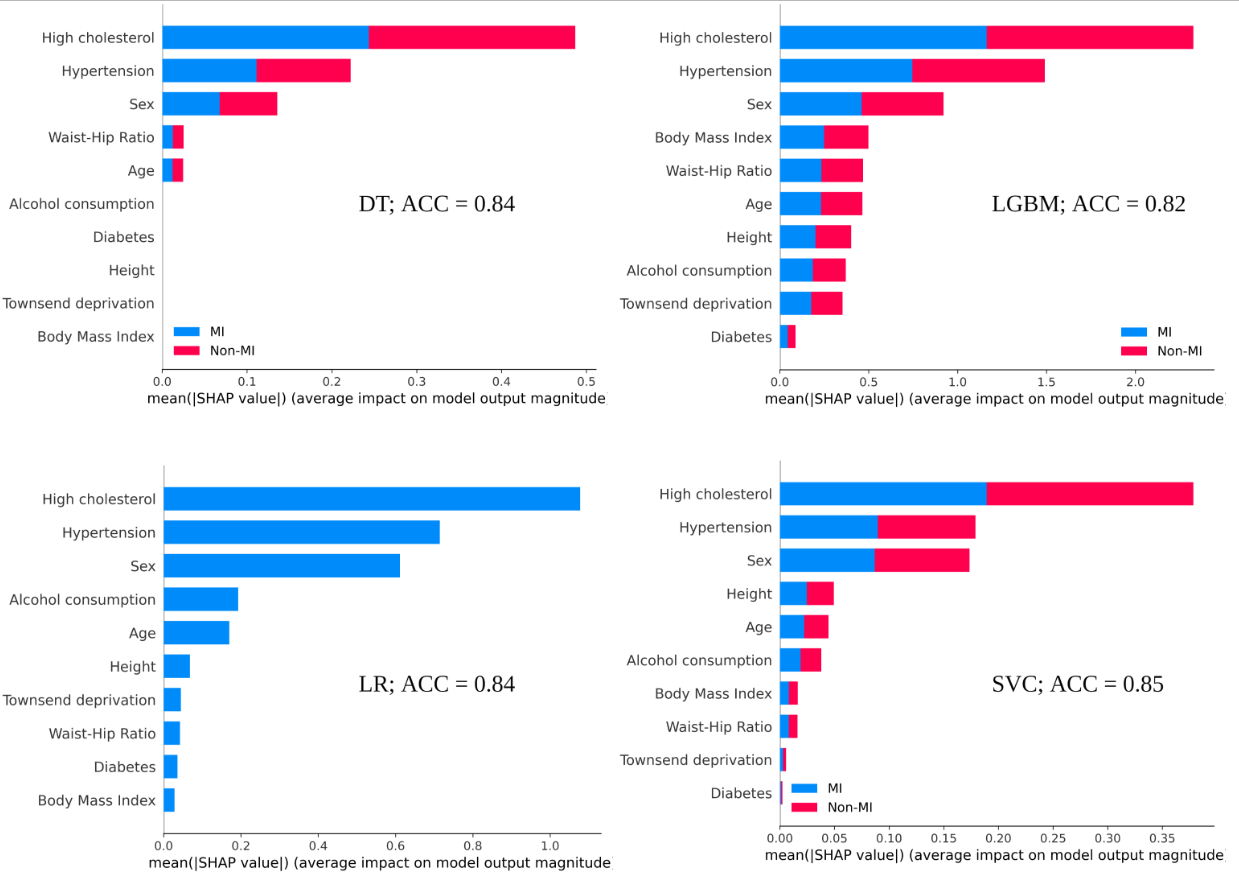
\includegraphics[width=\textwidth]{imgs/background/shap-example.png}
    \caption{\textit{SHAP output to explain four models globally. Models were applied to 1500 subjects (80\%/20\% train/test split) to classify them as cases (myocardial infarction, MI) or controls (No MI).  DT: decision tree; LGBM: light gradient-boosting machine; LR: logistic regression; SVC: support vector machines classifier; ACC: accuracy; MI: myocardial infarction.}}
    \label{fig:bg.xai.shapley}
\end{figure}
SHapely Additive exPlanation (SHAP) stands as a post-hoc, model-agnostic technique applicable to any machine learning model \cite{lundberg2017-shap}. Grounded in game theory, it assesses the contribution of each \say{player} to the overall \say{payout}. In the context of machine learning models, these \say{players} and the \say{payout} correspond to features and the model outcome, respectively. SHAP computes a score for each feature in the model, denoting its influence on the model's output. The calculation involves evaluating all possible combinations of features to cover scenarios where all features or a subset of features are in the model (\cref{fig:bg.xai.shapley}). As the number of features escalates, SHAP's computational complexity increases. To address this, an approximate SHAP method, Kernel SHAP, has been proposed. SHAP finds extensive applications across diverse domains to elucidate model outputs, whether on a local or global scale     (\cite{garcia2020-no2-shap,yesuel2022-heat-shap,ullah2023-grey-wolf}). Nonetheless, researchers and end-users should take note of certain aspects when employing SHAP. Primarily, SHAP is contingent on the specific model in use, i.e. model-dependent like LIME. This implies that the results obtained from SHAP can vary based on the model utilized, potentially resulting in differing explainability scores when employing different machine learning models.


\subsection{Explainability in GNNs}
\label{sec:bg.xai.gnn-xai}
After an overview of the interpretability/explainability sub-field of Machine Learning, a more detailed look on explainability techniques on graph neural network is presented, endorsing the main topic on which this text is focused on. Such an in-depth analysis will be needed regardless, given that the two explainability frameworks introduced in the previous section (\cref{sec:bg.xai.shap-lime}) have not been designed for graph data or deep models for graph.  

In recent times, the popularity of Graph Neural Networks (GNNs) has surged due to the prevalent representation of real-world data in graph formats. This includes data from various domains like social networks, chemical molecules, and financial data (see \cref{sec:bg.gnn.DL-on-graphs} for more examples). Several classification tasks on graph data tasks are widely studied, such as node classification \mycite{gao2019-graph-unets,henaff2015-deep-on-graph}, graph classification \mycite{xu2019-powerful,Zhang_Cui_Neumann_Chen_2018}, link predictions \mycite{zhang2018-link,cai2020-multi-scale}. Furthermore, numerous sophisticated operations for Graph Neural Networks (GNNs) have been introduced to enhance their performance. These encompass operations like graph convolution \cite{kipf2016-semisupervised}, graph attention \cite{veličković2018gat}, and graph pooling \cite{yuan2020-struct-pool}, that increase the overall complexity and illegibility.

However, compared with more common domains in deep learning, like images and text, the explainability of graph models is relatively less explored, critically damaging the overall understanding of deep graph neural networks. Recently, following the growing popularity of GNNs, several approaches have been proposed to explain their predictions. To name the most successful \mycite{xie2022-taskagnostic}, XGNN \mycite{yuan2020-xgnn}, GNNExplainer \mycite{ying2019-gnnexplainer}, PGExplainer \mycite{luo2020-pgexplainer}, and SubgraphX \mycite{yuan2021-subgraphx}, etc. These approaches have emerged from diverse perspectives, offering varying levels of explanations. Moreover, there is a current deficiency of standardized datasets and metrics to evaluate the results of explanations \mycite{yuan2022-xai-gnn-survey}.

To better understand these methods, the taxonomy of different explanation techniques for GNNs introduced in \mycite{yuan2022-xai-gnn-survey} can be followed. Based on what types of explanations are provided in output, the different methods can be classified into two main groups: instance-level methods and model-level methods. Overall, these two categories elucidate deep graph models from distinct perspectives. Instance-level methods furnish explanations specific to each example, whereas model-level methods offer overarching insights and a more general understanding. To validate and trust in most deep graph models, human oversight is still essential to review the explanations and give the correct interpretation of the explanation provided with those methods.

\paragraph{Instance-level methods}
\label{sec:bg.xai.instance-level}
According to the criterion used to obtain the explanations, Instance-level techniques can be categorized into four different branches: gradients/features-based methods, perturbation-based methods, decomposition methods, and surrogate methods.  

\begin{itemize}
    \item \textbf{Gradient/feature based methods} Utilizing gradients or features for explaining deep models is a common and direct approach, extensively applied in image and text tasks. The fundamental concept involves using gradients or values from hidden feature maps as approximations of input importance. In gradients-based methods \mycite{simonyan2014-deep,smilkov2017-smoothgrad}, the gradients of the target prediction concerning input features are computed through back-propagation. Conversely, in features-based methods \mycite{zhou2015-learning,selvaraju2019-gradcam}, hidden features are mapped back to the input space using interpolation to gauge importance scores. Given their simplicity and versatility, these methods can be straightforwardly extended to the graph domain. In recent times, numerous techniques have been employed to elucidate graph neural networks, such as SA, Guided BP \mycite{baldassarre2019-explainability}, CAM and Grad-CAM \mycite{pope2019-CVPR}. The principal distinction among these methods lies in the gradient backpropagation process and the manner in which diverse hidden feature maps are amalgamated.
    
    \item \textbf{Perturbation-based methods} These techniques find extensive use in explaining deep image models. The fundamental idea is to analyze how the outputs vary in response to diverse input perturbations. Essentially, if crucial input information is preserved, the predictions should remain akin to the original predictions. Current methods \mycite{dabkowski2017-saliency,yuan2020-discrete-masks,chen2018-learning}, involve training a generator to produce a mask that selects significant input pixels to expound deep image models. However, applying such techniques directly to graph models is not feasible. Unlike images, graphs are comprised of nodes and edges, and altering their dimensions to maintain uniform node and edge numbers is not possible. Generally perturbation-based methods are employed to derive masks from the input graph, highlighting crucial input features. It's important to note that varying types of masks are generated based on the explanation tasks, including node masks, edge masks, and node feature masks. Subsequently, the generated masks are integrated with the input graph, resulting in a modified graph that encapsulates essential input information. Finally, this updated graph is inputted into the trained GNNs for evaluating the masks and refining the mask generation algorithms. Many perturbation-based methods have been proposed over the last years, including GNNExplainer \mycite{ying2019-gnnexplainer}, ZORRO \mycite{funke2021-hard}, GraphMask \mycite{schlichtkrull2022-interpreting}, Causal Screening \mycite{wang2021-causal}, and SubgraphX \mycite{yuan2021-subgraphx}. 
    %%% TODO: riprendi dopo la softmax
    
    \item \textbf{Surrogate methods} The fundamental concept involves utilizing a straightforward and easy-to-understand surrogate model to approximate the predictions made by the intricate deep model for neighboring regions surrounding the input example. It's worth noting that these approaches operate under the assumption that relationships within the neighboring areas of the input example are less intricate and can be effectively represented by a simpler surrogate model. The explanations derived from this interpretable surrogate model are subsequently employed to elucidate the initial prediction. However, extending these surrogate methods to the graph domain presents challenges due to the discrete nature of graph data and the inclusion of topology information. In order to elucidate the prediction made for a particular input graph, the process begins by acquiring a local dataset that encompasses numerous neighboring data objects alongside their respective predictions. Subsequently, an interpretable model is trained on this local dataset to grasp the underlying patterns. The explanations derived from this interpretable model are then considered as explanations for the original model's prediction concerning the input graph. Some surrogate methods have been proposed recently to explain deep graph models, including GraphLime \mycite{huang2020-graphlime}, RelEx \mycite{zhang2021-relex}, and PGM-Explainer \mycite{vu2020-pgm-explainer}.
    
    \item \textbf{Decomposition methods} Another prevalent approach for explaining deep image classifiers involves decomposition methods. These techniques quantify the significance of input features by breaking down the original model predictions into distinct terms. These terms are subsequently considered as the importance scores corresponding to the respective input features. In this approach, a direct analysis of the model parameters is conducted to unveil the relationships between features in the input space and the resulting output predictions. It's important to emphasize that the conservative nature of these methods mandates that the sum of the decomposed terms equals the original prediction score. However, it is challenging to adapt such methods to the graph domain since graphs contain many components (e.g. nodes, edges, and node features), and it is non-trivial to distribute scores to different edges that may contain important structural information that should not be ignored. In these methodologies, the prediction score is propagated layer by layer using a backpropagation approach, extending all the way to the input layer. The process commences from the output layer, where the model's prediction serves as the initial target score. This score is then deconstructed and allocated to neurons in the preceding layer according to predefined decomposition rules. Through iteratively applying these steps until reaching the input space, significance scores for node features are acquired. These scores can be aggregated to signify edge importance, node importance, and walk importance. It's important to highlight that within these algorithms, the activation functions within deep graph models are overlooked. Common implementation of decomposition methods proposed to explain the deep graph neural networks include Layerwise Relevance Propagation (LRP) \mycite{baldassarre2019-explainability}, \mycite{schwarzenberg2019-layerwise}, Excitation BP \mycite{pope2019-CVPR} and GNN-LRP \mycite{schnake2022-high-order}.
    
\end{itemize}

\paragraph{Model-level methods}
\label{sec:bg.xai.model-level}
Diverging from instance-level methods, model-level methods strive to offer broader insights and a higher-level comprehension to elucidate deep graph models. In particular, they investigate the input graph patterns that influence specific behaviors in GNNs, such as optimizing for a particular prediction target. An established avenue within this realm is input optimization \mycite{olah2017-feat-viz}, which is widely used to derive model-level explanations for image classifiers. Although generalizing the explanations to a model-level perspective is a quite important and interesting improvement, at the time of writing this text only few works have tried to tackle this challenge. The few existing model-level method for explaining graph neural networks are XGNN \mycite{yuan2020-xgnn}, PGExplainer \mycite{luo2020-pgexplainer} which can be considered with perturbation-based methods (\cref{sec:bg.xai.instance-level}), and GCFExplainer \mycite{huang2023-globalCF} which employs counterfactual reasoning.

%\newpage
\subsection{Contrastive and counterfactual reasoning}
\label{sec:bg.xai.cf-reason}
The pursuit of human-centric AI has prompted extensive research into the essence of explanation. Nevertheless, a consensus regarding the definition of explanation remains elusive, even though explanation has garnered considerable attention, particularly within fields such as the philosophy of science \mycite{schurz2000-scientific-expl,pitt1989-theories-of-E}. In the context of AI, the broadest form of explanation typically relies on assessments of why an AI algorithm predicts a specific outcome and conjectures regarding the causes in relation to the observed effects \mycite{lombrozo2012-abductive-inferemce}. The necessity to produce explanations resembling those \say{generated} by humans has captured the interest of AI researchers, focusing on specific aspects of explanation and its sub-categories \mycite{miller2019-xai-insights}. Consequently, elucidating an algorithm's output in the context of plausible yet uncommon alternatives proves to be notably challenging, considering the potentially limitless array of such possibilities. Moreover, this complexity is compounded by the capacity to propose pertinent modifications to the input, resulting in a divergent decision by the algorithm, w.r.t. the original one.

With a growing focus on these forms of explanation, specifically referred to as \textit{contrastive} and \textit{counterfactual} within the XAI community, it becomes significantly important to examine the current theoretical explanations frameworks following this apporach for their automated generation \mycite{stepin2021-xai-cf-contrative-survey}. The interest here is even greater, considering that on such kind of XAI technique the research work presented in this text is based on. Thus, the aim of this section is to analyze relevant theoretical work on the contrastive and counterfactual accounts of explanation, and to discuss a degree of synergy between the revised theories and their related up-to-date implementations.

It's crucial to emphasize that contrastive explanations highlight the distinction between the actual decision and a hypothetical one. Conversely, counterfactual explanations outline the essential minimal alterations in the input required to produce a contrasting output. However, within the domain of XAI, these terms are at times used interchangeably \mycite{thai2020-grace,poyiadzi2020-face}. Diverse categories of techniques have been put forth to create both contrastive and counterfactual explanations for AI algorithm outputs. In the realm of XAI, when regarding an explanation for an automated decision or prediction as an observation, it can be abductively derived by engaging in a search process across the known information pertaining to that observation \mycite{bergadano2000-abduction}.

Whilst the generation of counterfactual explanations poses numerous technical challenges, it is imperative to consider various ethical dimensions. Primarily, there is an expectation that their usage is secure, as exposing the model's internal workings through counterfactuals could potentially facilitate model theft \mycite{sokol2019-counterfactualEO}. Additionally, counterfactual explanations should strive to be fair, ensuring that discriminatory explanations are avoided at all costs \mycite{kusner2018-counterfactual}. Moreover, these explanations should be actionable, meaning that the proposed alterations to the input should be practical and feasible \mycite{lucic2020-model-fail}. Lastly, accountability is a crucial aspect, emphasizing the need to ensure responsibility for the explanations furnished \mycite{arrieta2020-taxo-xai}.


\subsubsection{Contrastive explanations}
\label{sec:bg.xai.contrastive}
Accumulated insights from the humanities and social sciences regarding explanation demonstrate its inherent contrastive nature \mycite{miller2019-xai-insights}. This characteristic implies that an explanation addresses a \say{why} question concerning the cause of a specific event (\say{Why did $P$ happen}), considering hypothetical non-occurring alternatives (\say{Why did $P$ happen rather than $Q$?}) \mycite{lipton1990-LIPCE}. Therefore, proponents of the pragmatic explanation approach assert that the ability to distinguish the answer to an explanatory question from a set of contrastive hypothesized alternatives is what furnishes the explainee with sufficiently comprehensive insights into the rationale behind the question. Additionally, this approach establishes a fundamental criterion that an explanation must meet: it should assign higher probability to the observed event P compared to all hypothetical alternatives ($Q_1, Q_2, ..., Q_n$) \mycite{sormo2005-cased-based}.

The domain of cognitive science has been significantly impacted by the exploration of contrastive explanation \mycite{roese1997-cf-thinking,chinParker2017-ACA}. It is contended that contrastive explanations are an intrinsic part of human cognition \mycite{byrne2002-mental-models}. We naturally tend to question decisions we've previously made, particularly if these decisions or the accompanying circumstances led to tragic events \mycite{wenzlhuemer2009-cf-scientific}. Moreover, contrastive reasoning serves as the foundation for abductive inference \mycite{folger2016-abduction101}, where the objective is to infer specific facts that make certain observations plausible. Simply put, a particular observation can be elucidated by the most probable hypothesis among a set of competing alternatives \mycite{rappaport1996-inf-best}.

\subsubsection{Counterfactual explanations}
\label{sec:bg.xai.counterfactual}
Considering the inherent contrastive nature, one can envision alternative explanations for how things might have been if a different decision had been made at a certain point. This perspective can serve to explain potential consequences of such contrastive non-taken alternative decisions \mycite{stepin2021-xai-cf-contrative-survey}. In this scenario, it is assumed that the mind generates and juxtaposes mental representations of an event that actually occurred with those of an alternative event \mycite{byrne2015-cf-thought}. Cognitive scientists term these mental representations of alternatives to past events as counterfactuals (\say{contrary-to-fact}) \mycite{roese1997-cf-thinking}. Consequently, the process of contemplating 'past possibilities and present or past impossibilities' is referred to as counterfactual thinking \mycite{byrne1997-cognitivePI}. Furthermore, it is argued that counterfactual reasoning constitutes a fundamental mechanism for elucidating adaptive behavior in an evolving environment \mycite{paik2014-cf-reason-key,zhou2015-learning,zhang2015-reinforcement}.

Counterfactuals describe events or states of the world that did not occur and implicitly, or explicitly, contradict factual world knowledge. One definition of counterfactual \mycite{grahne1991-updates-and-cf} defines a counterfactual to be a conditional statement where the antecedent \say{can contradict the current state of affairs, or our current knowledge thereof}. Another interesting perspective is introduced by \mycite{ginsberg1986-counterfactuals}, they define counterfactual as a conditional statement of the form \say{If $P$, then $Q$} where $P$ is \say{expected} to be false.

In the broader computer science context, the veracity of a counterfactually deduced statement is determined by: (\textit{i}) creating a scenario where the most minimal alteration in the characteristics of the real world (as defined in the antecedent) results in a distinct (potentially desired) state of affairs (referred to as the \say{closest} or \say{nearest} conceivable world); and (\textit{ii}) gauging the accuracy of statements in that particular scenario \mycite{lewis1989-plurality-worlds}.

%%% TODO: add fast references to the CF expl for GNNs
%%% we analyze thos models in detail in the next chapter



%%%%%%%%%%%%%%%%%%%%%%%%% CHAP.3 : My method
\chapter[CFPGExplainer]{CFPGExplainer: Parametrized Counterfactual Explanations for Node Classification in Graph Neural Networks}
\label{chap:3-CFPG}
In this chapter we focus on the eXplainable Artificial Intelligence for Graph Neural Networks method that is the novelty introduce in this work: Counterfactual Parametrized Explaniner for graph neural network (CFPGExplainer). In section \ref{sec:cfpg.bg} we present an in-depth analysis of the XAI models that have mainly inspired our work, consequently we propose a formal definition (\cref{sec:cfpg.my.form-def}) for the research problem faced by CFPGExplainer. In the end of the chapter (\cref{sec:cfpg.my.archs}) we illustrate the architectural choices and the proposed approach implemented in the realization of our model.

\section{Related works}
\label{sec:cfpg.bg}
As introduced in the background section of this text (\cref{sec:bg.xai.gnn-xai}), despite the impressive success of GNNs on many predictive tasks, these models, coming as a direct evolution of deep networks on graph data, are black-box machine learning models. This means, as stated earlier, that is non-trivial to explain the rationale behind particular prediction made by a GNN, even though the ability to explain a model is critical towards making it trustworthy and thus suitable for many real-world applications. Owing to this limitation of GNNs, there has been significant efforts in recent times towards explanation approaches. 

In the next section we provide an in-depth look on the existing work on explaining GNN predictions that have mostly influenced this work: first of all GNNExplainer \mycite{ying2019-gnnexplainer} for introducing the concept of \say{explainer} for graph neural networks and for dealing with the lack of benchmark datasets for explanation tasks; PGExplainer \mycite{luo2020-pgexplainer}, being one of the first work trying to overcome the instance-level restrictions of graph network explainers; finally we take a closer look to CF-GNNExplainer \mycite{lucic2022-cfgnnexplainer} and GCFExplainer \mycite{huang2023-globalCF}, two of the most recent and interesting approaches, according to the authors of this text, to counterfactual explanations for GNNs. 

Lastly, an overview of the other works that have mostly influenced this thesis is provided. Especially over the graph generation methods \mycite{liu2019-cgvae,du2022-mdvae}, which provided many useful insights on the explanation generation step of this work, considering the similarity between the two tasks \mycite{zhu2022-survey-generation}, and the Graph Adversarial Attacks framework \mycite{bose2020-gaalvae}, taking inspiration from the analogies between counterfactual explanation and adversarial attacks on graph (additional details are provided in \cref{sec:cfpg.bg.graph-generation,sec:cfpg.bg.gaalv}). 


%%% Explainers for Graph Neural Networks
\subsubsection{Notation}
\label{sec:cfpg.bg.notation}
Before exploring the details of the explainer models of interest, here we briefly remind the notation to that is going to be used in the following paragraphs (\cref{sec:cfpg.bg.gnnexplainer,sec:cfpg.bg.pgexplainer,sec:cfpg.bg.cf-gnn,sec:cfpg.bg.globalCF}). Let $G$ denote a graph on edges $E$ and nodes $V$ ($G=(V,E)$) that are associated with $d$-dimensional node features $X = \{x_1 , . . . , x_n\}, x_i \in \mathbb{R}^d$ thus $X \in \mathbb{R}^{n\times d}$. The topology of the graph is encoded by the adjacency matrix $A \in \{0,1\}^{n\times n}$. And let $f(A, X; W ) \rightarrow y$ be any GNN, where $y$ is the set of possible predicted classes, and $W$ is the learned weight matrix of $f$. In other words, $A$ and $X$ are the inputs of $f$, and $f$ is parameterized by $W$. We note that later in this text input graphs and explanation subgraph are indicated directly with the symbol of the adjacency matrix $A$, given that it is the representation used for graph in practice in all the works analyzed in this section. 
Without loss of generality, we focus our examples on the problem of explaining a GNN model performing node classification task. Given a node $v \in V$ whose prediction we wish to explain, we denote by $G^c_v = (X^c_v, A^c_v)$ the computational subgraph of $f_{\theta}(G) = f(A, X; \theta)$. For example, for a three-layer Graph Convolutional Network (GCN, \cref{sec:bg.gnn.gcn}), $G^c_v$ contains all the neighbors up to order three described with the associated adjacency matrix $A^c_v \in \{0, 1\}^{n\times n}$ and their set of features $X^c_v = \{x_j | j \in X^c_v\}$.

%%% TODO: decidi se usare W o \theta per i parametri fi f(G)
%%% TODO: aggiungi notazione per computation subgraph, e perturbed adjaceny o perturbed node features

\subsection{GNNExplainer: Generating Explanations
for Graph Neural Networks} 
\label{sec:cfpg.bg.gnnexplainer}
\mycite{ying2019-gnnexplainer} employs soft masks for edges and node features to elucidate predictions through mask optimization. The process involves initializing soft masks randomly, treating them as trainable variables, and then combining these masks with the original graph using element-wise multiplications. Subsequently, the masks undergo optimization by maximizing mutual information between the predictions of the original graph and the newly obtained graph. Despite using various regularization terms, such as element-wise entropy, to guide the masks towards discreteness, they remain in a soft state, leading to the \say{introduced evidence} issue that GNNExplainer encounters. Moreover, the optimization of masks is specific to each input graph, potentially resulting in explanations lacking a holistic perspective.

A key insight in their work is the observation that the computation subgraph (considering that the adjacency matrix $A$ is the representation of the graph $G$) of node $v$ (denoted as $A_v^c$, or $A_v$ for the sake of simplicity), which is defined by the GNN’s neighborhood-based aggregation, fully determines all the information the GNN uses to generate prediction $\hat y$ at node $v$. The neighborhood-based aggregation considers that the node’s final representation only includes neighbors that are at most $k$ hops away from that node in the graph $G$, being $k$ the numbers of layers in the GNN. The rest of the nodes in $G$ are not relevant for the computation of the node’s final representation.

Moreover, \mycite{ying2019-gnnexplainer} introduced another important concept for this subfield of XAI. GNNExplainer provides the explanation of the prediction of a node $v$, as the subgraph $\hat{A}_v \subseteq A_v^c$, and the relative features $\hat{X}_v = \{x_j|v_j \in \hat{A}_v\}$, that are \say{important} for the GNN prediction. They formalize the notion of importance according to the mutual information ($MI$) criterion, formulated with conditional and joint entropy, i.e. the proposed method finds the explanatory subgraph and sub-features by maximizing the mutual information between the original prediction and the prediction based on the subgraph and sub-features. We can thus express GNNExplainer optimization framework as:
\begin{equation}
    \underset{A_s}{max} MI(Y_o,(\hat{A}_v,\hat{X}_v)) = H(Y_o) - H(Y_o| A = \hat{A}_v, X = \hat{X}_v)
    \label{eq:cfpg.bg.mutual-info-gnn}
\end{equation}
where $Y_o$ is the prediction of the GNN model with $A_o$ (the original unperturbed graph) as the input ($Y_o = f(A_o,X)$). For node $v$, $MI$ quantifies the change in the probability of prediction $\hat{y} = f(\hat{A}_v,\hat{X}_v)$ when $v$’s computation graph is limited to explanation subgraph $\hat{A}_v$ and its node features are limited to $\hat{X}_v$. It is worth noticing that $MI$ can serve, more generally, as a viable metric to evaluate the quality of internal representations within deep learning models; the information plane, in particular, offers valuable insights into whether the model effectively utilizes the accessible information present in the dataset \mycite{landsverk2022-mutual-info}.


\subsection{PGExplainer: Parameterized Explainer for Graph Neural Networks}
\label{sec:cfpg.bg.pgexplainer}
The method, proposed in \mycite{luo2020-pgexplainer}, learns approximated discrete masks over the edges to explain the GNN predictions. PGExplainer, together with GNNExplainer, belongs to the perturbation-based methods for XAI on graph neural networks (\cref{sec:bg.xai.instance-level}), but act on different components of the graph to induce the perturbation. Indeed PGExplainer produce the explanations perturbing only the structure of the graph, whereas GNNExplainer provides explanations on both structure and features (theoretically both edge and node features). This focus on structure stems from the similarity between feature explanation in GNNs and that in non-graph neural networks, a topic extensively explored in existing literature \mycite{guo2018-bayesian-non,lundberg2017-AUA,ribeiro2016-lime}.

For obtaining these edge masks, it adopts a deep neural network to parameterize the generation process of explanations, predicting the probability of each edge being selected (i.e. the probability of being in $\hat{A}_v$), which serves as the importance score. The process involves acquiring edge embeddings or, when edge feature are not available, concatenating embeddings of node incident to an edge, and then using these embeddings to make predictions. Subsequently, the approximated discrete masks are sampled using the reparameterization trick \mycite{niculae2023-discrete}. The training of the mask predictor network is carried out by maximizing the mutual information ($MI$) between the original predictions ($y = f(A,X)$) and the new predictions ($\hat{y} = f(\hat{A}_v,X_v)$), following the importance criterion introduced by (\cite{ying2019-gnnexplainer}, \cref{sec:cfpg.bg.gnnexplainer}). The optimization objective is thus comparable to what we showed in the previous paragraph for GNNExplainer, except for the absence of node features ($X_v$), given that PGExplainer strategy concerns only edge perturbation: 
\begin{equation}
    \underset{A_s}{max} MI(Y_o,\hat{A}_v) = H(Y_o) - H(Y_o| A = \hat{A}_v)
    \label{eq:cfpg.bg.mutual-info-pge}
\end{equation}

Although the reparameterization trick is utilized, resulting masks are not strictly discrete; however, they significantly mitigate the \say{introduced evidence} problem. Additionally, since a common predictor is shared by all edges in the dataset, the explanations can offer a comprehensive understanding of the trained GNNs. Indeed, compared to the existing work, PGExplainer has better generalization ability and can be utilized in an inductive setting easily. Such characteristic make this explainer one of the first, together with \mycite{yuan2020-xgnn}, facing the challenge of producing model-level explanations.   

\subsection{CF-GNNxplainer: Counterfactual Explanations for Graph Neural Networks}
\label{sec:cfpg.bg.cf-gnn}
Recently, as introduced in section \ref{sec:bg.xai.gnn-xai},there have been several attempts to extract explanations of graph neural networks (GNNs) via counterfactual reasoning \mycite{abrate2021-brain-networks,lucic2022-cfgnnexplainer,tan2022-learn-eval-cf,bajaj2022-robustCF}. In \mycite{abrate2021-brain-networks}, the authors explore counterfactual explanations within a more specialized category of graphs, namely brain networks \mycite{riedl2015-metabolicCM}, which consist of the same set of nodes. They employ a heuristic approach to iteratively add or remove edges in a greedy fashion. RCExplainer \mycite{bajaj2022-robustCF} aims to find a robust subset of edges whose removal changes the prediction of the remaining graph by modeling the implicit decision regions (considering the linear decision boundaries (LDBs), \cite{chu2018-exact-consistent}) based on GNN graph embeddings. More recently, the authors of CFF \mycite{tan2022-learn-eval-cf} argue that a good explanation for GNNs should consider both factual and counterfactual reasoning and they explicitly incorporate those objective functions when searching for the best explanatory subgraphs and sub-features.

We focus this supplementary analysis on one of the earlier methods considering counterfactual reasoning for GNN explanation, CF-GNNExplainer \mycite{lucic2022-cfgnnexplainer}, that provides counterfactual explanations in terms of a learnable perturbed adjacency matrix that leads to the flipping of classifier prediction for a node. The greatest improvement introduced by the authors with respect to existing methods for explaining the predictions of GNNs, that have primarily focused on generating subgraphs that are relevant for a particular prediction (\cite{yuan2020-xgnn,baldassarre2019-explainability,luo2020-pgexplainer,pope2019-CVPR,schlichtkrull2022-interpreting,ying2019-gnnexplainer,yuan2021-subgraphx,vu2020-pgm-explainer,lin2021-causal-expl}), is that CF-GNNExplainer is able to identify the minimal relevant subgraph automatically, whilst they all require the user to specify the size of the subgraph (i.e. the size of the explanation), $S$, in advance. The authors reveals that, even when adapting established methods for the counterfactual (CF) explanation challenge and experiment with different values for $S$, these methods fall short of generating valid, precise CF explanations. Consequently, they are not apt solutions for addressing the CF explanation problem.

The first intuition in their work is that we may want to change the relationships between instances (i.e. edges), rather than change the instances themselves (nodes), given that node feature may not be available. Therefore, a graph data CF example, for the prediction on node $v$, should have the form $\hat{v} = (\hat{A}_v, x)$, where $x$ is the feature vector of $v$ and $\hat{A}_v$ is a perturbed version of $A_v$, the adjacency matrix of the subgraph neighborhood of a node $v$. $\hat{A}_v$ is obtained by removing some edges from $A_v$ , such that $f(v) \ne f(\hat{v})$. Inspired by \mycite{wachter2018-GDPR}, \mycite{lucic2022-cfgnnexplainer}, they generate countefactcual examples by minimizing a loss function of the form:
\begin{equation}
    \mathcal{L} = \mathcal{L}_{pred}(v,\hat{v}|f,g) + \beta \mathcal{L}_{dist}(v,\hat{v}|d) 
    \label{eq:cfpg.bg.cfgnn-loss}
\end{equation}

where $f$ is the original GNN model, $g$ is the CF model, introduced in the article, that generates the CF example $\hat{v}$, and $\mathcal{L}_{pred}$ is a prediction loss (also referred to as miscalssification loss) that encourages the countefactual property ($f(v) \ne f(\hat{v})$). $\mathcal{L}_{dist}$ is a distance loss that encourages $\hat{v}$ to be \say{close} to $v$, and $\beta$ is a regularization coefficient that controls how important $\mathcal{L}_{dist}$ is compared to $\mathcal{L}_{pred}$. The two sub losses components are defined as:
\begin{align}
    \mathcal{L}_{pred}(v,\hat{v}|f,g) &= -\mathbb{1}[f(v) \ne f(\hat{v})] \cdot \mathcal{L}_{NLL}(f(v),g(\hat{v})) \\
    \mathcal{L}_{dist}(v,\hat{v}|d) &= dist(v,\hat{v})
\end{align}
\label{eq:cfpg.bg.cfgnn-losses}

where the negative sign in front of $\mathcal{L}_{pred}$ and the indicator function ensures the loss is active as long as $f(\hat{v}) = f(v)$. For the $dist$ function in $\mathcal{L}_{dist}$ any differentiable distance function can be considered. In (\cite{lucic2022-cfgnnexplainer}), they take $dist$ to be the element-wise difference between $v$ and $\hat{v}$ ($v \ominus \hat{v}$), corresponding to the difference $A_v \ominus \hat{A}_v$, i.e. the number of edges removed by the perturbation. This loss is tied on the CF model $g$, a GNN model trained to learn the perturbation matrix $P$ with the explanation objective described.
Despite of the novelties introduced by this first approach to counterfactual explanations for GNNs, CF-GNNExplainer is still an instance-based method, lacking the ability to generalize the CF examples to the whole dataset and provide an higher-level comprehension of deep graph models.


\subsection{GCFExplainer}
\label{sec:cfpg.bg.globalCF}
In \mycite{huang2023-globalCF} the authors propose the first method for \say{global} counterfactual explanations starting from the observation that most existing explainers for graphs (like \cite{vu2020-pgm-explainer,ying2019-gnnexplainer,yuan2020-xgnn}), both factual and counterfactual ones, provide instance-level explanation, considering a too narrow local perspective, generating counterfactual examples for individual input graphs. However, this kind of approach poses two key limitations: lacks global insights when working with multiple of data graphs; there can be an information overload owing to the number of counterfactual graphs growing linearly with the graph dataset size, significantly reducing the human-intelligible property highly desirable in XAI. 

Specifically, GCFExplainer aim to find a small set of representative counterfactual graphs that explains all input graphs, proposing an algorithm powered by vertex-reinforced random walks (VRRW, \cite{pemantle2004-vertexreinforced}) on an edit map of graphs with a greedy summary. The edit map ($\mathcal{G}$) is a meta-graph whose nodes are graphs in the same domain as the input graphs and edges connect graphs that differ by a single graph edit. $\mathcal{G}$ is used to organize the search space for counterfactual graphs in GCFExplainer, on which the random walks are performed. As an example, each graph in represents a node in the edit map, and the arrows denote edges between graphs (nodes) that are one edit away. VRRW has the nice property of converging to a set of nodes that are both \say{important} (i.e., cover many input graphs) and \say{diverse} (i.e., non-overlapping coverage), which will form a small set of counterfactual candidates for further processing.

In this very peculiar setting, although the vertex-reinforcement mechanism promotes diversity among heavily visited nodes, \mycite{huang2023-globalCF} introduce another formulation of the importance function, by assigning a large-edge\footnotemark weight $w(\bar{v},\bar{u})$ to good counterfactual candidates via an importance function $I(\bar{v})$:
\begin{equation}
    w(\bar{v},\bar{u}) = I(\bar{v})
\end{equation}

The importance function $I(\bar{v})$ is designed to capture the quality of a subgraph  as a counterfactual candidate. It has the following components: a counterfactual probability $p(\bar{v})$, that large-node $\bar{v}$ is a CF grah; an individial coverage measure ($\mathbf{coverage}(\bar{v})$ )that computes the proportion of input graphs that are close to $\bar{v}$; and a measure of the coverage gain ($\mathbf{gain}(v; \mathbb{S})$), when adding graph $\bar{v}$ to the current set of counterfactual candidates $\mathbb{S}$ (i.e., the n most frequently visited large nodes). 
\begin{equation}
    I(v) = p(\bar{v})(\alpha \mathbf{coverage}(\bar{v}) + (1-\alpha)\mathbf{gain}(\bar{v}; \mathbb{S}))
\end{equation}

where $\alpha$ is a hyperparameter between $0$ and $1$. Led by the above importance function, the VRRW method converges to a set of diverse nodes that have high counterfactual probability and collectively cover a large number of input graphs.

\footnotetext{With the prefix \say{large-} the authors of GCExplainer indicates the components of the edit map $\mathcal{G}$ that the random-walk explore \mycite{huang2023-globalCF}. Being meta-graph $\mathcal{G} = (\mathcal{V},\mathcal{E})$ a graph in turn, they talk about large-nodes ($\bar{v} \in \mathcal{V}$) and large-edges ($\bar{e} \in \mathcal{E}$).}


\subsection{Graph generation}
\label{sec:cfpg.bg.graph-generation}
In general, the task of graph generation is focused on computing hand-crafted statistical features of existing graphs with the purpose of generating new graphs with similar features. There are many real-world application for this task, for example, in drug discovery and chemical science, a fundamental yet challenging task is to generate novel, realistic molecular graphs with desired properties (e.g., high drug-likeness and synthesis accessibility, \cite{zang2020-moflow,jin2019-junction}). Traditionally graph generation models assume that real-world graphs obey certain statistical rules. However, this assumption oversimplifies the underlying distributions of graphs and is thus too strong to satisfy. As an illustration, the Barabási-Albert model \mycite{albert2002-barabasi} posits that similar graphs adhere to the same empirical degree distribution. However, this model falls short in capturing other essential elements, such as community structures, present in real-world graphs. Consequently, there is a growing interest in the development of deep models tailored for graph-structured data, as they facilitate the effective generation of complex graphs.

In the vast literature about graph generation \mycite{zhu2022-survey-generation}, our attention was attracted by two methods: Constrained Graph Variational Autoencoder (CGVAE, \cite{liu2019-cgvae}) and Monotonically Disentangled VAE (MD-VAE, \cite{du2022-mdvae}). The author of CGVAE were among the first to propose a probabilistic model for graph generation that builds gated graph neural networks (GGNNs, \cite{li2017-ggnn}) into the encoder and decoder of a variational autoencoder (VAE, \cite{Kingma2013-variational-bayes}) architecture. The graph generation framework of CGVAE follows a sequential approach to generation, starting from random nodes (\textit{focus} step) and generating the edge between them with the most probable class (\textit{expand}) step, in a graph-walk fashion order. The fundamental novelty in this work is that CGVAE is variational autoencoder model in which both encoder and decoder are graph-structured (i.e. graph neural network, GGNNs in this specific case). They also demonstrate how to incorporate hard domain-specific constraints to adapt the model for the molecule generation task. MD-VAE framework shares with CGVAE the intuition of using GNN models in the encoder and decoder roles of the VAE architecture. The main differences lie in how the molecule graph is generated, in (\cite{du2022-mdvae}) the generation is not sequential and is carried out through inference, and in the property control mechanism employed. In the work by (\cite{liu2019-cgvae}), the property control is performed at generation time, ensuring an higher validity for output molecules, but slowing down the whole process; whilst MD-VAE adopts the \textit{post-hoc} strategy of generating latent variables monotonically increasing, directly related to the specific characteristics desired for the output molecule. This is achieved with monotonic regularization, penalizing the violation of constraints via additional regularization terms together with the original objective.


\subsection{Generalizable Adversarial Attacks}
\label{sec:cfpg.bg.gaalv}
Another interesting point of view on explainable artificial intelligence comes from the cybersecurity perspective. It has been demonstrated in various settings, that the lack of interpretability and robustness of DNNs makes them vulnerable to adversarial attacks \mycite{sun2023-attack-defense}. For instance, \mycite{szegedy2014-intriguing} have pointed out the susceptibility of DNNs in image classification, proving how the performance of a well-trained DNN can be significantly degraded by adversarial examples, which are carefully crafted inputs with a small magnitude of perturbations added designed to fool prediction models. On the other hand it is also true that paying attention special attention to the security of deep network model can help satisfy the increasing need of developing trustworthy deep learning models. Thus, ensuring that a model has not been tampered with, and that its behavior is correct and faithful with respect to its design it is crucial to the proper application of explainability techniques.

Other than a mutual benefit in their recent exponential growth, the fields of XAI and Cybersecurity share some more characteristics. In machine learning, adversarial examples are inputs to ML models that an attacker has intentionally crafted by applying small but intentionally worst-case perturbations to examples from the dataset, such that the perturbed input results in the model outputting an incorrect answer with high confidence; they can be considered as optical illusions for machines \mycite{goodfellow2015-harnessing}. Taking a closer look inside the realm of XAI, the concept of counterfactual example tightly resembles that of adversarial example. If we consider perturbation-based approaches (\cref{sec:bg.xai.instance-level}) to explain deep graph models, the goal of those methods is to craft a small perturbation over input features (nodes) or structure (edges) that will result induce a change in final model prediction. Basically adversarial and counterfactual example can be seen as two sides of the same coin.

Building on this intuition, when designing the explainer proposed in this text, we took inspiration from the literature concerning adversarial attacks and defense techniques \mycite{sun2023-attack-defense}, specifically from the work of \cite{bose2020-gaalvae}. GAALV (Generelizable
Adversarial Attacks with Latent Variable perturbation mod-
eling) model offers a unified generative framework for whitebox adversarial attacks, which is easily adaptable to different input domains and can efficiently generate multiple adversarial perturbations. GAALV leverages advancements in deep generative modeling to learn an encoder-decoder based model with a stochastic latent variable that can be used to craft minimal perturbations. This framework brings forth several key benefits, main ones are: its domain agnostic nature, GAALV can be easily deployed in different domains (e.g., images, text, or graphs are tested in the original paper) by simply selecting the appropriate encoder, decoder, and similarity function for that domain; an efficient generalization, achieved employing a parametric model with a stochastic latent variable allows us to amortize the inference process when crafting adversarial examples; and finally the possibility to generate diverse by resampling attacks, when an initial attack fails. 

Without loss of generality, they define a generic adversarial generator network as a combination of four main components: a probabilistic encoder network, that defines a conditional distribution over latent encodings; probabilistic decoder network, that maps a sampled latent encoding to a perturbation; a combination function, that takes an input x and perturbation as input and outputs a perturbed example; and a similarity function, used to restrict the space of adversarial examples;

Even though this method is focused on perturbing node features, the generated perturbation influences $j$ nodes inside the neighborhood of the node $v$ whose prediction we want to taint (i.e. its computational subgraph $A^c_v$), contrasting with the subgraph (edge) perturbation proposed in our method (\cref{sec:cfpg.my.form-def}), and considered the previously mentioned similarity between CF and adversarial example, we took inspiration from GAALV framework to build our explainer model. 
Finally, given the different focus of this thesis, we refer the reader to the already cited, and the most comprehensive, at the time of writing this text, survey on adversarial attacks on graph data by \cite{sun2023-attack-defense}. 




\newpage
\section{Proposed Approach}
\label{sec:cfpg.my.archs}
In this section (\ref{sec:cfpg.my.archs}) we introduced the core of this thesis, the novel deep graph network explianer CFPGExplainer (\textbf{C}ounter\textbf{F}actual \textbf{P}arametrized \textbf{G}raph neural network \textbf{E}xplainer), a model-agnostic framework to generate counterfactual explanation for graph neural networks. With this method we aim to address some issues still present in the literature regarding explanation techniques for GNNs. First of all, the need to model-level CF explanations. To the best of our knowledge, the only works facing this challenge are GCExplainer \mycite{huang2023-globalCF} and RCExplainer \mycite{bajaj2022-robustCF}, that are capable of generalizing explanation at a model-level, but lack the ability to identify the minimal relevant subgraph automatically, forcing the user to specify the size of the explanation in advance, introducing an important bias on the final output and resulting in poorer performances. As stated in \cref{sec:cfpg.bg.cf-gnn}, CF-GNNExplainer (\cite{lucic2022-cfgnnexplainer}) instead resolve this issue, providing a framework that can identify the optimal exlpanation size, but that it is still bounded by its instance-level approach. 

Moreover, the efficiency in producing the countefactual examples, and explanation more in general, should be considered. Instance-level methods (\cref{sec:bg.xai.instance-level}), like CF-GNNExplainer and GNNExplainer \mycite{ying2019-gnnexplainer}, need to carry out a whole inference process for each node prediction one wish to explain, making the explaining process, overall, slower, other than tailoring the explanation to a very specific case. Furthermore, it is straightforward that the higher the number of nodes in a graph, and the higher its connectivity, the scalability of such methods could become a significant issue knowing taht various GNN based models have been applied to analyze graph data with millions of instances \mycite{ying2018-web-graphCN}. A solution to tackle this problem is offered by PGExplainer \mycite{luo2020-pgexplainer}, which adopting a deep neural network to parameterize the generation process of explanations (\cref{sec:cfpg.bg.pgexplainer}), enables a natural approach to explaining multiple instances collectively, and can be utilized in an inductive setting more easily than other strategies. This technique, although very promising, does not contemplate counterfactual reasoning, thus not enforcing all the benefits (\cref{sec:bg.xai.cf-reason}) that such a perspective on the XAI context has to offer. 

To briefly summarize, the following are the advatages of CFPGExplainer, the proposed explainer system:
\begin{itemize}
    \item \textbf{model-level explanations} we aim at providing the general insights and high-level understanding to explain deep graph models, with explanation not tailored to specific instances that can grasp a broader view of XAI tasks. 
    \item \textbf{efficient generalization} employing a parametric model with a stochastic latent variable allows us to amortize the inference process when crafting CF examples. In doing so, after training, we can efficiently generalize without any further optimization to unseen test examples with only a single pass through the trained explainer network.
    \item \textbf{counterfactual explanations} in many real-world applications producing an explanation in the form of the minimal input perturbation that result in an alternative output is way more meaningful than other approaches. For instance in drug discovery \mycite{stokes2020-antibiotic,xie2021-mars}, knowing why a molecule is predicted to not have a desirable property and what it lacks to achieve it, can help inform the design of new molecules and improve the understanding of molecular structures. 
\end{itemize}

\bigskip
\subsection{Problem form definition/formulation}
\label{sec:cfpg.my.form-def}
Following the notation in \cref{sec:cfpg.bg.notation}, we introduce in this section a more formal definition for the counterfactual explanation problem that the proposed CFPGExplainer aims to resolve.

In its most general form, a CF example $\hat{x}$ for an instance $x$ according to a trained classifier $f'$ is found by perturbing the features of $x$ such that $f'(\hat{x}) \ne f'(x)$ (\cite{wachter2018-GDPR}). 
For graph data, as seen in \cref{sec:bg.xai.gnn-xai}, it may not be enough to simply perturb node features, especially since they might not be always available. 
This is why we focus our attention in generating CF examples by perturbing the graph structure instead, considering also that the unique network structure of GNNs is the greatest peculiarity of these models. Therefore, in our setting, a counterfactual example $\hat{v}$ for the node prediction task performed by a GNN model $f_{\theta}(A,X)$ on a node $v$ is represented by the perturbed computational subgraph of $v$, $\hat{A}_v$. 
$\hat{A}_v$ is obtained by perturbing, i.e. removing some edges, from $A_v$ such that $f_{\theta}(\hat{A}_v,X_v) \ne f_{\theta}(A_v,X_v)$. 
The CFPGExplainer model computes the perturbation mask $P$, that when applied to $A_v$ produces $\hat{A}_v = P \otimes A_v$ (where $\otimes$ indicates the operation of removing the edges individuated by perturbation $P$). 
For the sake of simplicity, later in this section we denote $f_{\theta}(\hat{G}_v) = f(\hat{A}_v,X_v;\theta)$ and $f_{\theta}(G_v) = f(A_v,X_v;\theta)$, being $\hat{G}_v = (\hat{A}_v,X_v)$ and $G_v = (A_v,X_v)$ respectively. Following \mycite{lucic2022-cfgnnexplainer} we generate the counterfactual examples by minimizing a loss function of the form: 
\begin{equation}
    \mathcal{L} = \xi \cdot \mathcal{L}_{pred}(G_v,\hat{G}_v|f) + \beta \cdot \mathcal{L}_{size}(A_v,\hat{A}_v) + \gamma \cdot \mathcal{L}_{ent}(P) 
    \label{eq:cfpg.bg.cfpg-loss}
\end{equation}

where $\mathcal{L}_{pred}$ is a mis-classification loss that encourages the final perturbation to produce a counterfactual example ($f(G_v) \ne f(\hat{G}_v)$). $\mathcal{L}_{size}$ is a term to enforces the the perturbation to be minimal, penalizing the loss when the explanation size grows. $\mathcal{L}_{ent}$ serves to reduce the entropy in the values of the perturbation mask. Finally $\xi$, $\beta$ and $\gamma$ are regularization coefficient to control the importance of each term in $\mathcal{L}$.

More in detail we do not want $f(G_v)$ to match $f(\hat{G}_v)$ to enforce the counterfactual property, thus we put a negative sign in front of $\mathcal{L}_{pred}$ and include an indicator function to ensure the loss is active as long as $f(G_v) \ne f(\hat{G}_v)$:
\begin{equation}
    \mathcal{L}_{pred}(G_v,\hat{G}_v|f) = -\mathbb{1}[f(G_v) \ne f(\hat{G}_v)] \cdot \mathcal{L}_{NLL}(f(G_v),f(\hat{G}_v)))
\end{equation}

$\mathcal{L}_{size}$ is the number of edges removed by the perturbation, essentially the element-wise difference between $A_v$ and $\hat{A}_v$: 
\begin{equation}
    \mathcal{L}_{size}(A_v,\hat{A}_v) = dist(A_v,\hat{A}_v) = A_v \ominus \hat{A}_v 
\end{equation}

The last term $\mathcal{L}_{ent}$ is a binary entropy loss \mycite{Goodfellow-et-al-2016} computed over all the elements of $P$, since each $\rho \in P$ represents the probability of each edge to be part of the perturbation (note that $N_P = |P|$):
\begin{equation}
    \mathcal{L}_{ent}(P) = - \frac{1}{N_P} \sum_{\rho \in P} \rho \cdot log(\rho) + (1 - \rho)\cdot log(1 - \rho)]
\end{equation}

%Having introduce this consideration we show the complete formulation of the learning objective terms: 
%\begin{align}
%    \mathcal{L}_{pred}(G_v,\hat{G}_v|f) &= -\mathbb{1}[f(G_v) \ne f(\hat{G}_v)] \cdot \mathcal{L}_{NLL}(f(G_v),f(\hat{G}_v))) \\
%    \mathcal{L}_{size}(A_v,\hat{A}_v) &= dist(A_v,\hat{A}_v) \\
%    \mathcal{L}_{ent}(P) &= - \frac{1}{N_{P}} \sum_{\rho \in P} \rho \cdot log(\rho) + (1 - \rho)\cdot log(1 - \rho)]
%\end{align}
%\label{eq:cfpg.bg.cfpg-all-losses}

\bigskip
\paragraph{Reparametrization trick}
\label{sec:cfpg.my.discrete-latent}
Nonetheless, directly optimizing the aforementioned objective function becomes infeasible due to the presence of $2^m$ (we remind that $m = |E|$) potential candidates for $\hat{A}_v$.
Thus, we need to consider a relaxation by assuming that the explanatory graph is a Gilbert random graph \mycite{gilbert1959-random-graphs}, where selections of edges from the original input graph $A_o$ are conditionally independent to each other.

Because $\hat{A}_v$ is discrete in nature, we relax edge weights from binary variables to continuous variables in the range $(0, 1)$ and adopt the reparameterization trick to efficiently optimize the objective function with gradient-based methods \mycite{jang2017-gumbel}. Categorical variables are a natural choice for representing discrete structure in the
world, for this reason, following \mycite{luo2020-pgexplainer} we adopt the Gumbel-Softmax, a continuous distribution on the simplex that can approximate categorical samples, and whose parameter gradients can be easily computed via the reparameterization trick, and thus integrated into neural networks and trained using standard backpropagation \mycite{niculae2023-discrete}. The problem of discrete latent structures classification in neural networks can be tackled with various techniques, and in this work some test have been performed using sparsemax \mycite{martins2016-sparsemax}. Sparsemax is a sparse alternative to softmax that corresponds to regularizing the argmax with the Gini entropy \mycite{ross2007-intro-prob}. 
Unlike the softmax function, sparsemax does not necessarily eliminate sparse points, and it can even yield a vertex, especially when the disparity between the highest and second-highest scores is sufficiently substantial. This behavior mirrors the margin property found in max-margin losses when applied in a latent context \mycite{blondel2020-fenchel-young,niculae2023-discrete}.


%\bigskip
\subsection{Explainer architecture}
\label{sec:cfpg.my.model}
We now introduce our method CFPGxplainer, as stated in the beginning of this chapter (\cref{chap:3-CFPG}), its workflow and architecture, and summarize its details in \cref{fig:cfpg.my.cfpg-model}. Note that in the following description we are assuming that both the explainer model and the GNN model heve been already trained on the tasks of generating the perturbation mask and node classification raspectively. 
Given a node $v$ in the test set, we first obtain its original prediction $y_o$ from GNN model $f$, as $y_o = f_{\theta}(A_v,X_v)$, next we run CFPGExplainer to compute the perturbation mask $P$ and obtain the perturbed computation subgraph of $v$, $\hat{A}_v = P \otimes A_v$. 
Having $\hat{A}_v$ we execute again the GNN to be explained to see if the perturbation is sufficient to induce a change in the final prediction, using the pertrurbed adjacency we compute $\hat{y} = f_{\theta}(\hat{A}_v,X_v)$. At this point, if $\hat{y} \ne y_o$, we have produced a valid counterfactual example for $v$, $\hat{v} = \hat{A}_v$. The following picture illustrates the general process, just described, to generate counterfactual examples. 
\bigskip
\begin{figure}[h]
    \centering
    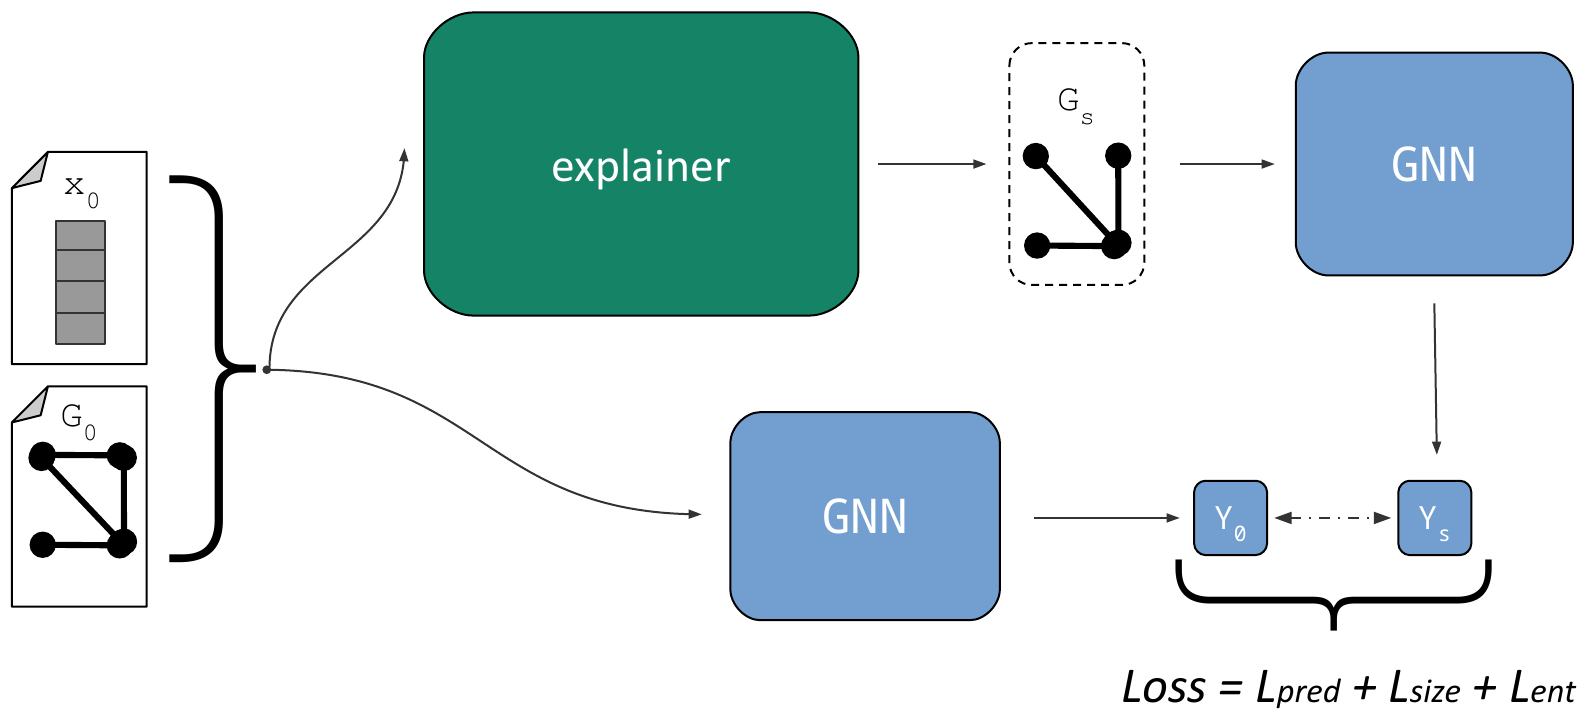
\includegraphics[width=\textwidth]{imgs/cfpg/cfpg-general-02.png}
    \caption{\textit{The CFPGExplainer method general pipeline. The raw input data $A_o,X_o$, node feature and adjacency matrix respectively, are initially fed both to the explainer and to the GNN model.}}
    \label{fig:cfpg.my.cfpg-model}
\end{figure}



\paragraph{Explainer inner working}
\label{sec:cfpg.my.cfpg-inner}
The explainer module (\cref{fig:cfpg.my.cfpg-inner}) processes the input data executing three main steps: an encoding phase, a decoding phase and a sampling phase. First the input data fed through a three-layer GCN model to get an encoded representation that takes into account the structure of the graph, inspired by the many works in graph generation literature that exploit this strategy \mycite{zhu2022-survey-generation}, especially those works focused on deep generative models based on Variational AutoEncoders (VAEs). The key intuition in this step is that this \say{parallel} GCN model is trained following the counterfactual learning objective (\cref{eq:cfpg.bg.cfpg-loss}). We chose to implement three layer of graph convolution so that the \say{parallel} model can be aware of the same computational subgraph $A^c_v$) the primary GNN model is aware, as in \mycite{ying2019-gnnexplainer}, that is to say the 3-hop neighborhood in this precise instantiation.

The second phase consists of crafting edge representations (a sort of inner embeddings) for those edges that constitute the computational subgraph of a node, the ones involved by the explanation analysis, and subsequently feeding them into two fully connected layers that are supposed to learn to assign to each edge the probability of being part of the explanation. Following \mycite{luo2020-pgexplainer} edge embeddings are built concatenating the embeddings of the nodes connected by each edge, and the embedding of the node whose prediction we are explaining, together. Thus, when explaining the prediction of $v$, to craft the embedding of edge $e = (u,w), e \in A^c_v$, we concatenate the embeddings of $v,u,w$, namely $x_v,x_u,x_w \in X$, and obtain $e' = (x_v \cup x_u \cup x_w)$.
%%% TODO: metti immagine corretta dell'architettura
\begin{figure}[h]
    \centering
    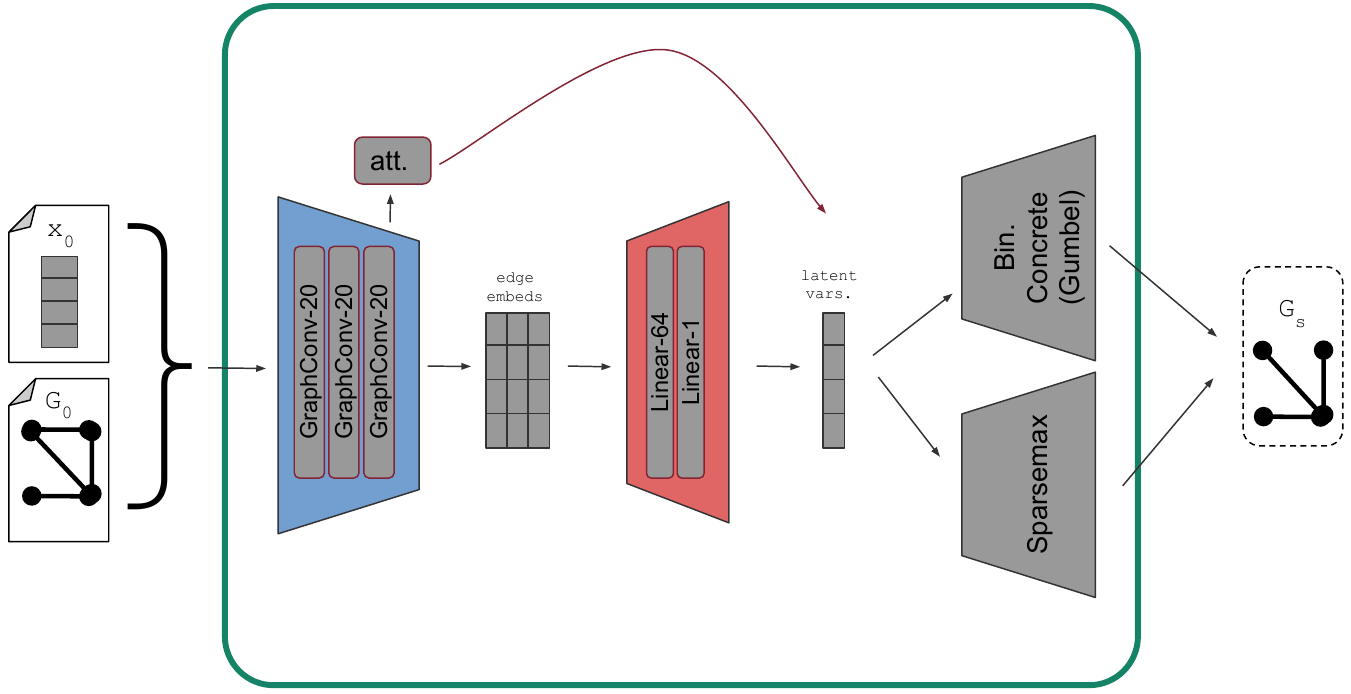
\includegraphics[width=\textwidth]{imgs/cfpg/cfpg-schema-fake.png}
    \caption{\textit{A close-up look to CFPGExplainer inner workings. The picture shows two options for the final sample phase to resemble the two strategies we have tested in this research. Note that the actual model implements one sampling module at a time.}}
    \label{fig:cfpg.my.cfpg-inner}
\end{figure}

Lastly, in the third sampling phase, we sample a random graph, the perturbation $P$, from edge distributions acquired in the second phase, that is then combined to $A^c_v$ to produce its perturbed version $\hat{A}_v$ (i.e. the CF example) that can thus be fed again to the trained GNN model to get the masked prediction. To conclude this final step, we employ categorical reparametrization with gumbel-softmax (\cref{sec:cfpg.my.discrete-latent}, \cite{jang2017-gumbel}). 
It is noteworthy that in order to seamlessly conclude a single training step the primary GNN model must be previously trained and the original prediction for each node in the training and testing portion of the dataset should be computed in advance, as the model solely requires only the final prediction value.   



%%%%%%%%%%%%%%%%%%%%%%%%% CHAP.4 : Experiments
\chapter{Experimental setup}
\label{chap:4-expRes}
In this chapter we illustrate the experimental settings in which our proposed explainer model has been tested. First we dive in a small introduction of the synthetic dataset developed for specifically for explanation tasks (\cref{sec:expRes.syns-dataset}), and real-world data that are suitable for this purpose (\cref{sec:expRes.real-dataset}). In \cref{sec:expRes.cf-metrics} we provide an overview of the metrics that should be adopted in a counterfactual XAI context, and finally in \cref{sec:expRes.res} we present the results of our experiments with CFPGExplainer.

\paragraph{Software and hardware setup}
\label{sec:expRes.setup}
The piece of software written to test empirically CFPGExplainer has been developed in python, version 3.10 \mycite{vanRossum2009-python} relying on the Pytorch\footnote{\url{https://pytorch.org/}} machine learning framework \mycite{pytorch2019-NEURIPS}, on the PYtorch-Geometric\footnote{\url{https://pytorch-geometric.readthedocs.io/en/latest/index.html}} libraries specifically designed for geometric deep learning (PyG, \cite{fey2019-PyG}); and on NVIDIA CUDA libraries (version 11.7) for GPU processing \mycite{cudaToolkit}. All experiments have been executed on a laptop machine running a linux operating system (Ubuntu\footnote{\url{https://www.ubuntu-it.org/}} 22.04) with 16GB of RAM and 2GB of VRAM.  

%%% TODO: see XAI taxo survey for datasets
\section{Synthetic datasets}
\label{sec:expRes.syns-dataset}
In recent times, there has been an emergence of synthetic datasets tailored for evaluating explanation techniques (\cite{ying2019-gnnexplainer,luo2020-pgexplainer}). In such datasets, different graph motifs are included and can determine the node labels or graph labels. Furthermore, the relationships between data examples and their respective labels are meticulously defined by human experts. Even though the trained GNNs may not perfectly capture such relationships, the graph motifs can be employed as reasonable approximations of the ground truths of explanation results. Here we introduce the most widely used synthetic datasets in GNN explanation tasks.

\paragraph{BA-shapes}
\label{sec:expRes.ba-shapes}
(syn1): It is a node classification dataset with 4 different node labels. It contains a base graph (300 nodes) and a house-like five-node motif (one for the top of the house, two in the middle, and two on the bottom). 
Note that the base graph is obtained by the Barabási-Albert (BA) model, which can generate random scale-free networks with a preferential attachment mechanism \mycite{albert2002-barabasi}. 
The motif is attached to the base graph while random edges are added. Each node is labeled based on whether it belongs to the base graph or different spatial locations of the motif: there are four possible classes (not in-motif, in-motif top, in-motif middle, in-motif bottom) 
- indices of expl. labeled nodes: $[300,700)$ every 5;

\paragraph{BA-community}
\label{sec:expRes.ba-comms}
(syn2): a node classification dataset with 8 different labels. Each graph is obtained by combining two BA-shapes graphs with randomly added edges. Node labels are determined by the memberships of BA-shapes graphs and their structural locations. The memberships of the BA-shapes graphs and the structural location determine the labels.  
- indices of expl. labeled nodes: $[300,700) \cup [1000,1400)$ every 5; 

\paragraph{Tree-Cycles}
\label{sec:expRes.tree-cycles}
(syn3): It is a node classification dataset with 2 different labels. Each graph it consists of a base balanced tree graph with the depth equal to 8 and a six-node cycle motif. These two components are randomly connected. The label for the nodes in based graphs is 0 otherwise 1.
- indices of expl. labeled nodes: $[511,871)$ every 6;

\paragraph{Tree-Grids}
\label{sec:expRes.tree-grids}
(syn4):  It is a node classification dataset with 2 different labels. It is the same as the Tree-Cycle dataset, except that the Tree-Grids dataset employs nine-node ($3\times 3$) grid motifs instead of cycle motifs.
- indices of expl. labeled nodes: $[511,1231)$ every 3/9;

\paragraph{BA-2Motifs}
\label{sec:expRes.ba-2motifs}
It is a graph classification dataset with 2 different graph labels. There are 800 graphs and each of them is obtained by attaching different motifs, such as the house-like motif and the five-node (BA-shapes, \cref{sec:expRes.ba-shapes}) cycle motif (Tree-Cycle, \cref{sec:expRes.tree-cycles}), to the base BA graph. Different graphs are labeled based on the type of motif.

\subsection{Real-world datasets}
\label{sec:expRes.real-dataset}
%\subsection{Molecule datasets}
%\label{sec:expRes.molecule-dataset}

\paragraph{Molecule datasets}
\label{sec:expRes.mutag}
Molecular datasets are also widely used in explanation tasks, such as MUTAG \mycite{debnath1991-mutag}, BBBP \mycite{martins2012-BBBP}, and Tox21 \mycite{wu2018-moleculenet}. Each graph within these datasets is a representation of a molecule, with nodes symbolizing atoms and edges denoting the chemical bonds. The labeling of molecular graphs is typically derived from the chemical functionalities or properties inherent to the molecules. Utilizing these datasets for explanation tasks demands domain-specific knowledge, such as an understanding of which chemical groups serve as discriminative factors for their functionalities.

MUTAG molecular dataset is the most common dataset for XAI tasks. It contains several molecules represented as graphs where nodes represent atoms and edges chemical bonds. The molecules are labelled based on their mutagenic effect on a specific bacterium \mycite{debnath1991-mutag}. Carbon rings with chemical groups $NH_2$ or $NO_2$ are present in mutagenic molecules, and are known to lead to mutagenic effects.
The task performed here is binary graph classification (mutagenic,non-mutagenic) and good explainer should identify such patterns for the corresponding class. Obviously MUTAG, as well as all the molecular dataset cited here, is not a synthetic dataset, but is reported here due to many work in XAI for GNNs (\cite{ying2019-gnnexplainer,luo2020-pgexplainer,spinelli2022-mate-maml}) using it as one of the few real-world dataset containing explanation ground truth values.


\paragraph{Text datasets}
\label{sec:expRes.text-data}
Text data proves to be a suitable choice for graph explanation tasks because it comprises words and phrases with readily understandable semantic meanings. Consequently, the results of explanations can be easily assessed by humans. Thus, we have constructed three sentiment graph datasets based on text sentiment analysis data, encompassing the SST2, SST5 \mycite{socher2013-SST2-5}, and Twitter \mycite{dong2014-twitter} datasets.

Initially, for each text sequence, we transform it into a graph in which each node represents a word, and the edges signify relationships between different words. To accomplish this, we leverage the Biaffine parser \mycite{gardner2018-allennlp} for extracting word dependencies. In Figure 5, we provide an example of one of the sentiment graphs we've generated. It's worth noting that these generated graphs are directed, although we omit edge labels, as most Graph Neural Networks (GNNs) are incapable of capturing edge label information. Subsequently, we employ BERT \mycite{devlin2018-bert} to acquire word embeddings, and these embeddings serve as the initial representations for the graph nodes. Specifically, we utilize a pre-trained twelve-layer base BERT model to extract a 768-dimensional feature vector for each word.
%\section{Preprocessing}
%\label{sec:expRes.preprocessing}
%Property of the European Southern Observatory...

\bigskip
\section{Countefactual metrics}
\label{sec:expRes.cf-metrics}
Although visualization results can offer valuable insights into the human perspective on the reasonableness of explanations, these assessments are not entirely reliable due to the absence of established ground truths. Moreover, comparing various explanation methods necessitates human examination of results for each input example, which is a time-consuming process. Furthermore, human evaluations tend to be highly subjective and may lack fairness.
Hence, the significance of evaluation metrics in the study of explanation methods becomes evident. Effective metrics should appraise the results from the model's standpoint, gauging factors like the faithfulness of explanations to the model \mycite{jacovi2020-faithfully,wiegreffe2019-attention-notnot}. This section will introduce several recently developed evaluation metrics tailored for explanation tasks, as introduce in \mycite{arrieta2020-taxo-xai}.


\paragraph{Fidelity} 
\label{sec:expRes.fidelity}
In tasks involving factual explanations, it is imperative that the explanations faithfully represent the model's perspective. They ought to pinpoint the input features that hold significance for the model, rather than being tailored to human preferences or understanding.
In literature, Fidelity is defined as the proportion of nodes where the original predictions match the prediction for the explanations (\cite{molnar2022,ribeiro2016-lime}). Since we are dealing with the counterfactual task of generating counterfactual (CF) examples, our objective is to ensure that the original prediction does not align with the prediction made for the explanation. Therefore, we aim for a low fidelity value in this context. As shown by \mycite{amara2022-graphFramEx}, this definition of fidelity can be extended by considering in addition the explanation focus, making some adjustments: when it comes to the phenomenon focus, fidelity is assessed in relation to the ground-truth node label. On the other hand, for the model focus, it is evaluated with regard to the GNN model's output.


\paragraph{Explanation Size}
\label{sec:expRes.expl-size}
In this setting the size of the explanation is the number of removed edges. This metric corresponds to the $\mathcal{L}_{size}$ term in \cref{eq:cfpg.bg.cfpg-loss}, which represents the disparity between the original $A_v$ and the counterfactual $\hat{A}_v$. In our quest for concise explanations, our aim is to minimize this metric, seeking a smaller value. It's important to note that we cannot apply this metric to evaluate GNNExplainer like models (\cite{luo2020-pgexplainer,yuan2020-xgnn,vu2020-pgm-explainer,bajaj2022-robustCF}), since they need the user to indicate the explanation size in advance, making this perspective useless.


\paragraph{Sparsity}
\label{sec:expRes.sparsity}
Effective explanations should also exhibit sparsity, signifying their ability to encompass the most critical input features while disregarding irrelevant ones. The Sparsity metric quantifies this characteristic by gauging the proportion of features identified as important by explanation methods \mycite{pope2019-CVPR}.
More specifically, sparsity measures the proportion of edges in $A^c_v$ that are removed (Yuan et al., 2020b). A value of $0$ indicates all edges in $A^c_v$ were removed. Given our preference for succinct explanations, we aim for a value approaching $1$ for this metric. Note that, also in this case, we cannot evaluate this metric for GNNExplainer like models as for explanation size (\cref{sec:expRes.expl-size}), for the same problem in their approach to generating explanation.


\paragraph{Accuracy}
\label{sec:expRes.accuracy}
Additionally, the Accuracy metric has been introduced for synthetic datasets \mycite{ying2019-gnnexplainer,sanchez2020-attributeGNNs}. In the case of synthetic datasets, even if it remains uncertain whether GNNs make predictions as expected, the principles underlying the construction of these datasets, including graph motifs, can serve as reasonably close approximations of ground truths. Consequently, for any given input graph, we can assess its explanations in relation to these ground truths. For instance, when examining significant edges, we can evaluate the concordance rate between the important edges in explanations and those present in the ground truths.

In the context of this study, accuracy is defined as the average proportion of explanations that are deemed \say{correct}. In line with the methodology established by \mycite{ying2019-gnnexplainer,luo2020-pgexplainer}, accuracy is computed exclusively for nodes that were originally predicted to be part of the motifs. This restriction is imposed because accuracy can only be reliably calculated for instances where we have knowledge of the ground truth explanations.
As we strive for concise explanations, we classify an explanation as \say{correct} if it exclusively encompasses edges that are contained within the motifs, meaning it only removes edges that are situated within the motifs.


\newpage
\section{Results}
\label{sec:expRes.res}
In this section we present the results of the experiments executed in this study. First, the focus of our model, CFPGExplainer (\cref{chap:3-CFPG}), is to explain node classification task in GNNs, thus all the following results have been obtained considering the synthetic datasets (\cref{sec:expRes.syns-dataset}) for node classification. Following \mycite{luo2020-pgexplainer} and\mycite{spinelli2022-mate-maml}), for the sake of simplicity, we have adopted some aliases in developing the code and crafting the results tables; later in this text we say: \texttt{syn1} as BA-shapes, \texttt{syn2} as BA-community, \texttt{syn3} as Tree-Cycles and \texttt{syn4} as Tree-Grids.

%%% tabella con i risultati del training della GNN su tutti i dataset 

%%% tabella con gli hyper-parametri per le configurazioni ottimali

%%% tabella con i risultati degli explainer su tutti i dataset



%%%%%%%%%%%%%%%%%%%%%%%%% CHAP.5 : Conclusions
\chapter{Conclusions}
\label{chap:5-conclusions} 
The grasping power of the mirror..

%%% TODO: citare adv-attack, graph generation as future works



\backmatter
\cleardoublepage % blank page after each chapter

%%%%%%%%%%%%%%%%%%%%%%%%% bibliography
\phantomsection % Give this command only if hyperref is loaded
\addcontentsline{toc}{chapter}{\bibname}
% Here put the code for the bibliography. You can use BibTeX or
% the BibLaTeX package or the simple environment thebibliography.
\printbibheading
\printbibliography[type=article,heading=subbibliography,title={Articles}]
\printbibliography[type=inbook,heading=subbibliography,title={Inproceedings}]
\printbibliography[type=book,heading=subbibliography,title={Books}]
\printbibliography[type=misc,heading=subbibliography,title={Miscellaneous}]

\end{document}